
\documentclass[phd,tocprelim]{cornell}

\let\ifpdf\relax
\usepackage{url}
\usepackage{graphicx}
\usepackage{color}
\usepackage{float}

\usepackage[section]{placeins}
\usepackage{graphicx,pstricks}
\usepackage{graphics}

\usepackage{moreverb}
\usepackage{subfigure}
\usepackage{epsfig}
\usepackage{txfonts}
\usepackage{multirow}
\usepackage{todonotes}
\usepackage{glossaries}
\usepackage[none]{hyphenat}
\usepackage{setspace}
\usepackage{hyperref}
\usepackage{listings}
\usepackage{minted}



\graphicspath{ {Images/} }

\usepackage[utf8]{inputenc}

\tolerance=9999


\bibliographystyle{plain}
%\bibliographystyle{IEEEbib}

\usepackage{listings}
\usepackage{color}

\makeglossaries

\definecolor{lightgrey}{rgb}{236,236,236}
\definecolor{dkgreen}{rgb}{0,0.6,0}
\definecolor{gray}{rgb}{0.5,0.5,0.5}
\definecolor{mauve}{rgb}{0.58,0,0.82}
\renewcommand{\topfraction}{0.85}
\renewcommand{\textfraction}{0.1}
\renewcommand{\floatpagefraction}{0.75}
\renewcommand{\chaptername}{Kapittel}
\renewcommand{\abstractname}{Sammendrag}
\renewcommand{\acknowledgements}{Takk}
\renewcommand*\listfigurename{Figurliste}
\renewcommand\listoflistingscaption{Kodeliste}
\renewcommand{\bibname}{Referanser}

\title{Forbedret brukervennlighet innen alternativ og supplerende kommunikasjon for mennesker med forsinket 
eller avvikende språk- og kommunikasjonsutvikling} 

\author{Morten Holst Øvrebø / }

\begin{document}

\begin{figure}[ht!]
\centering

\includegraphics[width=80mm]{HIB_sort_hovedlogo_engelsk}
\end{figure}


\maketitle

%\section*{Forord}


\begin{abstract}

Denne rapporten tar for seg prosessen rundt utviklingen av en high-fidelity prototype basert på en eksisterende programvare og testing av nye funksjoner for økt brukervennlighet. 

Tobii Dynavox har en programvare som heter Sono Flex som skal hjelpe unge mennesker som helt eller delvis mangler tale å kommunisere ved hjelp av øyesporing. De ønsket å utforske to ting.  Muligheten for å utvikle programvaren på en mer moderne plattform. Implementere og teste hvilke påvirkning animasjoner og lyd har på målgruppen.

Programvaren ble bygget på en ny plattform med hovedfunksjonaliteten tilgjengelig. Koden har følgt en såpass god standard at det skal være mulig å videreutvikle den til et en fullstendig programvare. I tilegg til hovedfunksjonaliteten ble det også implementert flere animasjoner. 

Til slutt ble det også utført en test på programvaren. Denne ga ikke nok data til å konkludere hvorvidt animasjoner og lyd ga økt brukevennlighet, men nok til at en person kan bruke den til kommunikasjon.



1
\end{abstract}


\begin{Acknowledgements}


Tusen takk til Tobii Dynavox som har hjulpet med å fullføre denne rapporten. Med en spesiell takk til Morten Mjelde fra Tobii, for gode ideer og tilbakemeldinger gjennom oppgavetiden. 

En stor takk til mine veiledere Harald Soleim, Atle Geitung, Remy Monsen og Jon Eivind Vatne for veiledning jeg ikke kunne ha greid meg uten.

For hjelp til å rekruttere testere vil jeg takke Solveig Kalgraf og Marie Brandvoll Haukenes ved HiB og Anne Moen ved pedagogisk-psykologiske tjenesten i Arna. For gjennomføring og tillatelse til å teste på Krohnengen barneskole ønsker jeg å rette en stor takk til Monica Storvik.

Til slutt ønsker jeg å vise takknemlighet til barna som deltok i testen og til deres foreldre for tillatelse.

\end{Acknowledgements}




\newglossaryentry{isaac}{name=ISAAC, description={ International Society for Augmentative and Alternative Communication}}

 \newglossaryentry{aske}{name=ASK, description={Alternativ og Supplerende kommunikasjon}}
 
  \newglossaryentry{PCCR}{name=PCCR, description={Pupil Centre Cornea Reflection, er en teknikk som brukes til ikke-forstyrrende øyesporing}}

  \newglossaryentry{WPF}{name=WPF, description={Windows  Presentation  Foundation}}
  \newglossaryentry{XAML}{name=XAML, description={Extensible Application Markup Language}}
 
\printglossary[title=Ordliste, toctitle=Beskrivelse av ord og forkortelser]
\contentspage
\figurelistpage
\listoflistings

\normalspacing \setcounter{page}{1} \pagenumbering{arabic}
\pagestyle{cornell} \addtolength{\parskip}{0.5\baselineskip}



\chapter{Introduksjon}




\section{Bakgrunn}
\label{sec:motivasjon}

Tale og språk tillater oss å rekke ut til andre og leve tilfredsstillende liv som uavhengige medlemmer av samfunnet. Språk gir oss identitet, felleskap og tilhørighet. Det er derimot flere som blir hindret i å uttrykke seg gjennom tradisjonelle kommunikasjonsformer på grunn av ulike funksjonshemninger  \cite{tobii}. De har derfor et behov for alternativer, for å kunne kommunisere. Folk med syn eller hørselsskader har tatt i bruk gester, tegnstøtte eller tegnspråk. Andre har måttet bruke mer håndgripelige hjelpemidler. Ett kjennetegn ved disse formene for kommunikasjon er at de krever at brukeren har muskelkraft. Et krav som utelukker  personer med ALS, cerebral parese (CP), autisme og afasi eller de som har hatt hjerneslag. Folk med disse funksjonshemningene har ofte motoriske utfordringer som hindrer dem fra nettopp verbal og kroppsspråklig kommunikasjon. Ved hjelp av data- og øyestyrings-teknologi er det mulig for flere av disse menneskene å kommunisere. Utfordringen er at feltet er relativt ungt og nåværende forskning har hovedsakelig blitt gjort på voksne uten funksjonshemninger \cite{aac}. I dette prosjektet vil fokus bli rettet mot barn som ikke har tilgang på tradisjonelle kommunikasjonsformer. 


\section{Motivasjon}
\label{sec:goal}

I dette prosjektet skal vi lage et digitalt ASK-system som hjelper barn med komplekse kommunikasjonsbehov å kommunisere. Systemet som skal utvikles tar utgangspunkt i et eksisterende program som heter Sono Flex (se figur ~\ref{fig:SonoFlex}). Programmets hovedfunksjon er å konvertere tekst og symboler til tale, men inneholder også et rikholdig utvalg av funksjoner for læring, omgivelseskontroll og elektronisk fjernkommunikasjon \cite{TobiiCommunicator}. Formålet med systemet er å hjelpe brukeren å kommunisere med symboler. Der et symbol representerer et ord eller et konsept som "hjem" eller "min mor". 

Sono Flex fungerer svært bra, problemstillingen er at når brukerens aktive vokabular vokser, så vil også antallet symboler øke. Dette gjør at det oppstår et behov for å dele symbolene inn i kategorier og flere visninger. Et barn vil da måtte navigere gjennom flere sider for å kunne skrive en ønsket setning. Noe som kan være belastende på et barn.

Light og Drager \cite{aac} argumenterer at videre forskning innen ASK teknologi må fokusere på forbedret design, for bedre å kunne møte behovet fra unge barn og eldre nybegynnere. I dette prosjektet er målet å designe og prototype mulige løsninger som reduserer den mentale belastningen på brukeren, mens han bruker et stort vokabular, med eller uten en øyestyrings enhet. 

\begin{figure}[ht!]
\centering
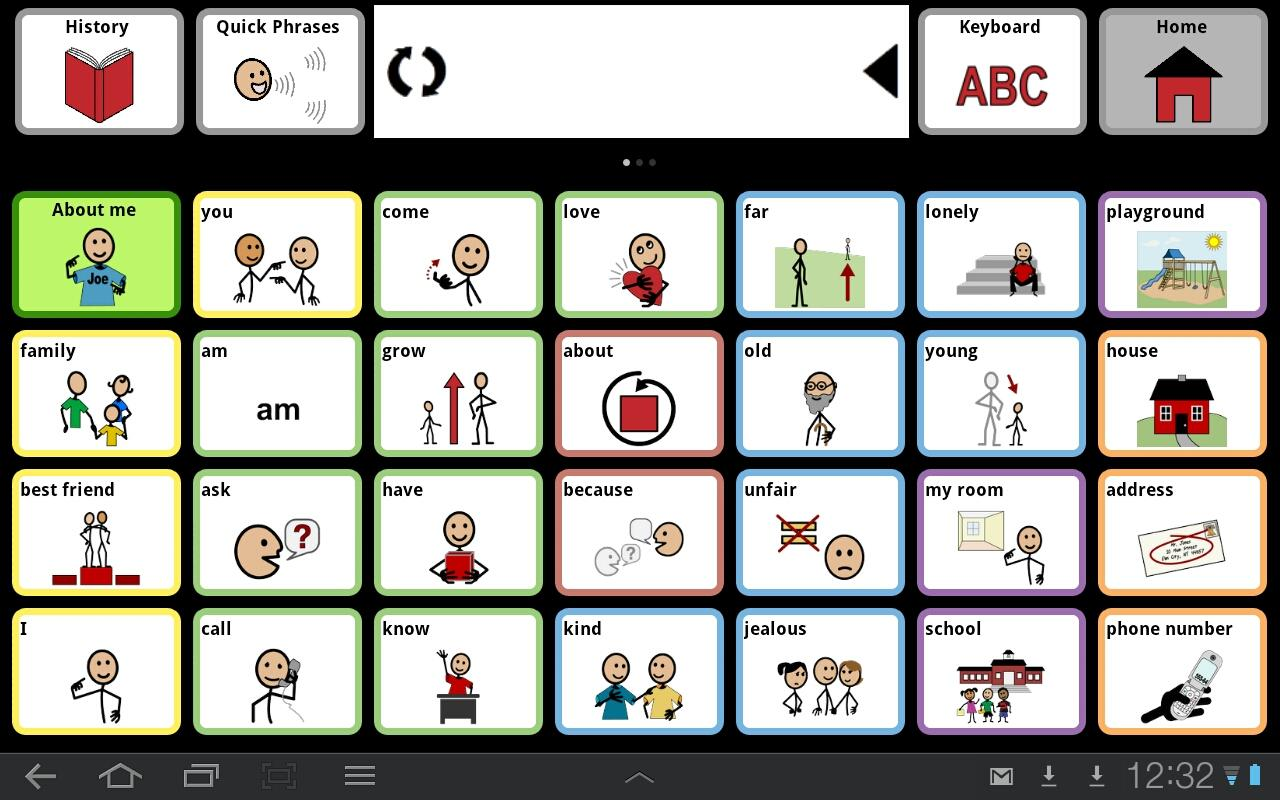
\includegraphics[width=150mm]{SonoFlex2}
\caption{Skjermdump av ASK programvaren Sono Flex}
\label{fig:SonoFlex}
\end{figure}


\section{Målsetninger}

Utgangspunktet til oppgaven var å se på måter enn kunne forbedre designet til Sono Flex. Det ble derimot tidlig i startfasen etablert at Tobii ikke ønsket at utviklingen skulle skje på deres eksisterende kode. Grunnen er at den eksisterende teknologien som programvaren er bygget på begynner å bli utdatert. Den eksisterende teknologien og koden er i god stand, men ikke optimal for de ønskede forbedringene. 

Målet med oppgaven har derfor blitt todelt. Det vil si at i tillegg til å bygge ut funksjoner og teste disse på den eksisterende programvaren, vil også programvaren som disse skal fungere på utvikles. Første delmål av oppgaven vil derfor være å utvikle programvaren. Andre delmål vil være å teste ulike design og funksjoner.

\subsection{Første delmål: Prototype}

På grunn av begrenset med tid og ressurser ville det ikke være mulig  utvikle en fullverdig versjon av den eksisterende løsningen Sono Flex. Planen ble derfor å bygge en high-fidelity prototype hvor kun hovedfunksjonaliteten var prioritert.  

Når en først skulle starte et nytt prosjekt ble det bestemt at det burde fokuseres på kodekvalitet. God kode hadde uansett vært i fokus, men i denne sammenheng menes det litt utover det. Slik at istedenfor å kun ha hovedfokus på å implementere funksjonalitet, så bør den være implementert slik at den følger standarder og mønster. Tankegangen var at ved å gjøre dette ville det være mulig å bruke prototypen i fremtidige prosjekter. Det økte også muligheten for at prototypen kunne videreutvikles til et ferdig prosjekt. 

Minstekravet til prototypen var at den skulle gi brukeren mulighet til å sette sammen enkle setninger å spille disse av som lyd. De ulike ordene skulle bli delt inn i tilhørende kategori. Hvis det ble tid skulle det også være mulig for en bruker og tilpasse programvaren. Som forskjellige fargetemaer, symbolstørrelse, animasjonsfart o.s.v.


\subsection{Andre delmål: Forbedret brukervennlighet}
\label{sec:ResearchQuestion}

For å utforske mulige løsninger som kan øke brukervennligheten til Sono Flex vil en rekke funksjoner og design implementeres og testes. Først skal vi se på hvordan animasjon og lyd kan hjelpe en bruker i å finne ønsket symbol raskere. Deretter ønsket vi å finne en måte å gjøre det mulig for en bruker å endre innstillinger kun ved å bruke øyene. Vi velger å kalle dette øyestyrt brukertilpasning. Til slutt vil vi utforske veier en kan organisere og kategorisere ord på, for å best legge tilrette for et barn. Listen nedenfor gir en  beskrivelse av det vi ønsker å utforske.

\begin{enumerate} 
\label{lst:features}
\item Animasjon. Undersøk mulige fordeler forskjellige visualisering effekter kan ha på navigering innen og mellom sider og kategorier.
\item Lydeffekter. Undersøk mulige fordeler forskjellige lydeffekter kan ha på navigering innen og mellom sider og kategorier.
\item Optimal organisering og kategorisering. Hvordan skal knapper bli organisert og kategorisert for best å legge til rette for og forenkle navigasjon
\item Brukertilpasning. Mennesker har forskjellige preferanser, derfor er det i de fleste programvarer mulig for en bruker å tilpasse etter ønske. I dette tilfelle ønsker vi å gjøre dette mulig gjennom øyestyring. Spesifikk vil vi se på mulighetene for tilpasning av symbolstørrelse, animasjonsfart, farger og generelle innstillinger. 
\end{enumerate}

Forskningen vil bli gjort ved å implementere et program basert på en eksisterende løsning. De ulike forbedringene beskrevet i listen vil bli integrert.

\section{Testing}

Som nevnt i seksjon \ref{sec:ResearchQuestion}, er oppgaven å forbedre en type kommunikasjons programvare for mennesker med komplekse kommunikasjonsvansker. For å undersøke innvirkningene til de forskjellige funksjonene, vil de prøves ut på en testgruppe. For å få til dette, vil et utvalg av deltakerne prøve systemet uten tilleggsfunksjonene, mens de gjenværende vil forsøke med funksjonene. Mens deltagerne kjører programmet vil deres interaksjon med bli automatisk lagret i logg. Informasjonen fra undersøkelsen vil vise hvordan brukeren navigerte og hvor lang tid de brukte. Dette kan igjen brukes til å verifisere om en funksjon er en forbedring eller ikke.

\subsection{Målgruppe}

I kapittel \ref{sec:motivasjon} nevnes det at det er flere unge mennesker som helt eller delvis mangler tale. Som en konsekvens av dette har de behov for andre uttrykksformer for å kommunisere. Alternative uttrykksformer kan være håndtegn, symboler eller fotografier. Slike utradisjonelle uttrykksformer går under fellesbetegnelsen alternativ og supplerende kommunikasjon (\gls{aske}).
Personer bruker ASK enten fordi det er et behov for å erstatte talen eller for å supplere utydelig eller svak tale.

International Society for Augmentative and Alternative Communication (\gls{isaac}) \cite{HvaErASK} definerer ASK som alt som hjelper en person til å kommunisere effektivt når tradisjonelle måter å kommunisere på ikke strekker til.

Målgruppen er personer som har behov for ASK systemer. Mer spesifikk vil programvaren være rettet mot: (A) Mennesker som ikke har mulighet for tale- og kroppsspråk,  (B) personer ikke håndterer skriftspråk og (C) at de er nybegynnere på symbolbasert kommunikasjon. Dette gjelder hovedsakelig barn i alderen 2 til 5 år, men også eldre med mentale begrensninger. Videre i dette prosjektet vil personer som møter disse kriteriene bli omtalt som barn med komplekse kommunikasjonsbehov. 


\section{Oppsummering}

Tobii Dynavox vil utforske potensielle forbedringer i deres programvare. Problemet er at den eksisterende teknologien ikke er tilstrekkelig. Dette gjør at før vi kan utvikle og teste mulige forbedringer, må en prototype utvikles. Målet for oppgaven blir derfor først å utvikle prototype, deretter implementere mulige forbedringer.
Finnes ikke så mye bakgrunns materiale, har tatt med det som finnes. Vil nok ta mest tid å utvikle programvaren
 
\chapter{Bakgrunn}
I dette kapittelet vil vi gå dypere inn i hva vi ønsker å finne ut og hvordan vi skal prøve å finne dette ut. 


\section{Tidligere Forskning}

\subsection{Organisering}

I 1926 kartla Smith\cite{Smith} barns vokabularutvikling fra alderen 1 til 5 år . Resultatene (se tabell \ref{fig:BarnVak}) viste at allerede i en alder av 3 er det vanlig å ha en gjennomsnittlig forståelse for cirka 900 ord. Forskningen er 88 år gammel, men viser omfanget av utfordringen barn har i møte med symbolbasert kommunikasjon. Mens et barn med taleevne kun trenger å finne ordet i hukommelsen, må barn som bruker symboler først finne det og deretter lokalisere det representative symbolet. 

I applikasjonen som skal utvikles vil symbolene bli presentert i en tabell. Antall symboler som får plass i tabellen begrenses av skjermens fysiske størrelse og at de må være store nok til at brukeren har mulighet til å se  og samhandle med dem. En slik tabell med symboler vil herfra bli referert til som en side. For hver setning brukeren vil uttrykke må han navigere seg igjennom flere av disse sidene for å finne symbolene som representerer ordene i setningen. Det er derfor essensielt at organiseringen legger til rette for akkurat dette, og ikke vanskeliggjør barnets evne til å lokalisere, velge og bruke symbolene.

\begin{table}[h]
\begin{tabular}{llllllllll}
\hline
Alder (År, Måneder) & 1 & 1,6 & 1,9 & 2,0 & 2,6 & 3,0 & 3,6  & 4,0  & 5,0  \\ 
Antall ord          & 3 & 22  & 118 & 272 & 446 & 896 & 1222 & 1540 & 2072 \\ 
Økning              & 2 & 19  & 96  & 154 & 174 & 450 & 326  & 330  & 532  \\ \hline
\end{tabular}
\caption{Tabell som viser vokabular vekst hos barn.  Smith \cite{Smith} sitert av Dale \cite{Dale} }
\label{fig:BarnVak}
\end{table}


Drager og Light \cite{aac} viser til at det inntil nylig var gjort lite forskning på layouts og organisering for barn eller om faktorene som spiller inn når det gjelder lokalisering og bruk av målobjektene. Målobjektet er symbolet som brukeren ønsker å uttrykke. Wilkinson og Jageroo \cite{Wilkinson2006} har undersøkt hvilke påvirkning farge har som en faktor når det kommer til organisering og hvordan elementer skal fordeles. De kom frem til at fargehint spiller en viktig rolle innen visuell prosessering  og hukommelse. Ved å legge til en farge ved elementene i tabellen over symboler, påvirket det nøyaktigheten og effektiviteten til barn i 4-5 års alderene i å finne målobjekt. Eksempelvis kan man gi symboler som representerer verb en grønn farge, adjektiv en blå, pronomen gul o.s.v. Fenomenet kalles Fitzergald Key og gjør at barn mer presist og raskere lokalisere målobjektet. Scally \cite{Scally} argumenterer for at farge ikke nødvendigvis er den eneste variabelen som må vurderes. Andre skjerm variabler som kan påvirke læring og bruk er: bakgrunn, kanter/grenser, form, tekstur, størrelse, posisjon, bevegelse og animasjon. Videre undersøkelser må til for å avgrense effektene av disse funksjonene for å kunne optimere designet til ask-systemer.


\subsection{Navigasjon}
\label{subsec:navigasjon}

Hvis en tar med alle typene frukt så vil det ikke være plass til alle symbolene på en side, dette gjør at de må deles opp over flere sider.Konsekvensen er at brukeren må ha mulighet til å navigere mellom disse sidene for å finne ønsket symbol. Siden antallet symboler det er plass til på hver side begrenses av skjermstørrelsen og brukerens syn, er spørsmålet hvor mange symboler bør plasseres på hver side med tanke på effektivitet. Drager og light med kollegaer undersøkte nettopp dette. Resultatene indikerte at barn i alderen 2-5 hadde større vanskeligheter for å lokalisere korrekt side fra en meny med 4 symboler enn en så lokalisere målobjektet når på korrekt side ut av et valg på 12 til 30 symboler, til tross for at sannsynligheten for å finne korrekt side er 25 prosent er mye større enn å finne korrekt symbol 0.03 - 0.08 når en først er på rett side.

For barn kan det å navigere være ekstra vanskelig. Dette kommer av flere grunner: (a) de må ha en konseptuell modell av de gjemte sidene i systemet i minnet. Med andre ord forstå hvordan de mest effektivt kan komme seg fra forsiden til ønsket symbol. (b) De må forstå forholdet mellom representasjon brukt på menysiden og de gjemte sidene i vokabularet. Er det symbolet med bilde av et kjøkken eller av en butikk som leder til symbolet eple? I denne rapporten vil disse utfordringene bli undersøkt.





\chapter{Tobii Sono Flex}
I dette kapittelet vil den eksisterende løsningen Sono Flex bli presentert. 

\section{Tobii Sono Flex}
\label{chap:Tobii-Sono-Flex}

Programvaren som det tas utgangspunkt i heter Tobii Sono flex,  og er et systematisert symbolforråd og et verktøy for alternativ og supplerende symbolspråk. Sono flex har som mål å tilby et språk til personer som ikke enda kan lese og skrive. 

Applikasjonen fungerer som et tastatur, men istedenfor bokstaver er knappene ord med en visuell representasjon av ordet. Brukeren trykker på knappene som utgjør setningen han vil uttrykke,  programvaren vil da gjøre om setningen til tydelig tale. Systemet er spesielt utviklet for barn og unge med med sammensatte kommunikasjonsvansker som trenger et ordforråd for å videreutvikle språk- og kommunikasjonsferdigheter. 

Sono flex kan ses på som en nybegynnerpakke med en lav læringskurve som skal gjøre brukeren klar for mer avanserte systemer. Det vil si at den skal lære brukeren to ting, La brukeren bygge et vokabular og vende seg til å bruke øyesporing.


\subsection{Brukergrensesnitt}

Brukergrensesnittet til Sono flex består av to hoveddeler: en menylinje og en symboltabell. 


\subsubsection{Menylinje}

Figur \ref{fig:menylinje} viser menylinjen, som består av 5 elementer. Det hvite feltet i midten viser symbolene som brukerene har trykket på, og vil herved bli referert til som setningslisten. Symbolene som vises vil komme ut i form av tydelig tale ved å trykke på selve feltet. Knappen på venstre side av setningslisten (clear all), vil ved interaksjon tømme setningslisten. Mens knappen på høyre side vil kun fjerne det siste symbolet brukeren trykket på.


\begin{figure}[ht!]
\centering
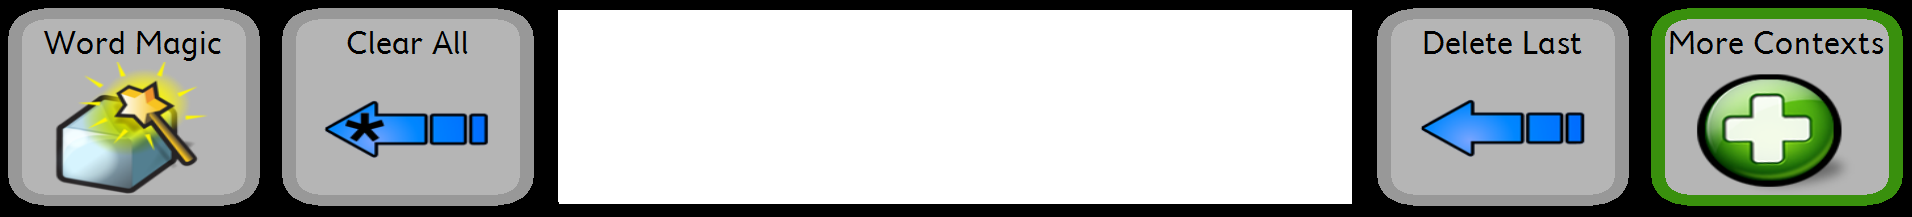
\includegraphics[width=100mm]{menylinje}
\caption{Menylinjen til programvaren Sono flex}
\label{fig:menylinje}
\end{figure}


\subsubsection{Symboltabell}
\label{subsubsec:symboltabell}

Figur \ref{fig:symbolgrid} viser applikasjonens symboltabell. Dette komponenten består av en tabell på 7 kolonner og 4 rader, noe som gir 28 celler totalt. I hver celle er det en knapp bestående av et symbol og en tekstlig beskrivelse av symbolet. Ved å trykke på knappen vil en av tre hendelser inntreffe avhengig av hvilken type symbol det er. De tre typene er ord-,kategori- og navigasjons-symbol.

Hvis knappen representerer et ord ( "jeg",  "løpe",  "kake" o.s.v. ) vil det være et ordsymbol. Ved å trykke på knappen vil symbolet og medfølgende tekst vises i setningslisten i menylinjen.

Hvis symboler har underliggende symboler som eksempelvis en ordklasse (verb,  substantiv)  eller kategori ("mat",  "frukt") vil det være et kategori symbol. Ved å trykke på knappen vil applikasjonen bytte ut de eksisterende symbolene i tabellen med ordene i ordklassen. 

Den siste typen symbol, er et navigasjonssymbol. Denne forekommer kun hvis det er for mange symboler i forhold til hvor mange det er plass til. Dersom en kategori inneholder flere symboler enn tabellstørrelsen, må symbolene fordeles over flere sider. Navigasjonssymbolet vil da være tilstede for å kunne bla mellom de ulike sidene.


\begin{figure}[ht!]
\centering
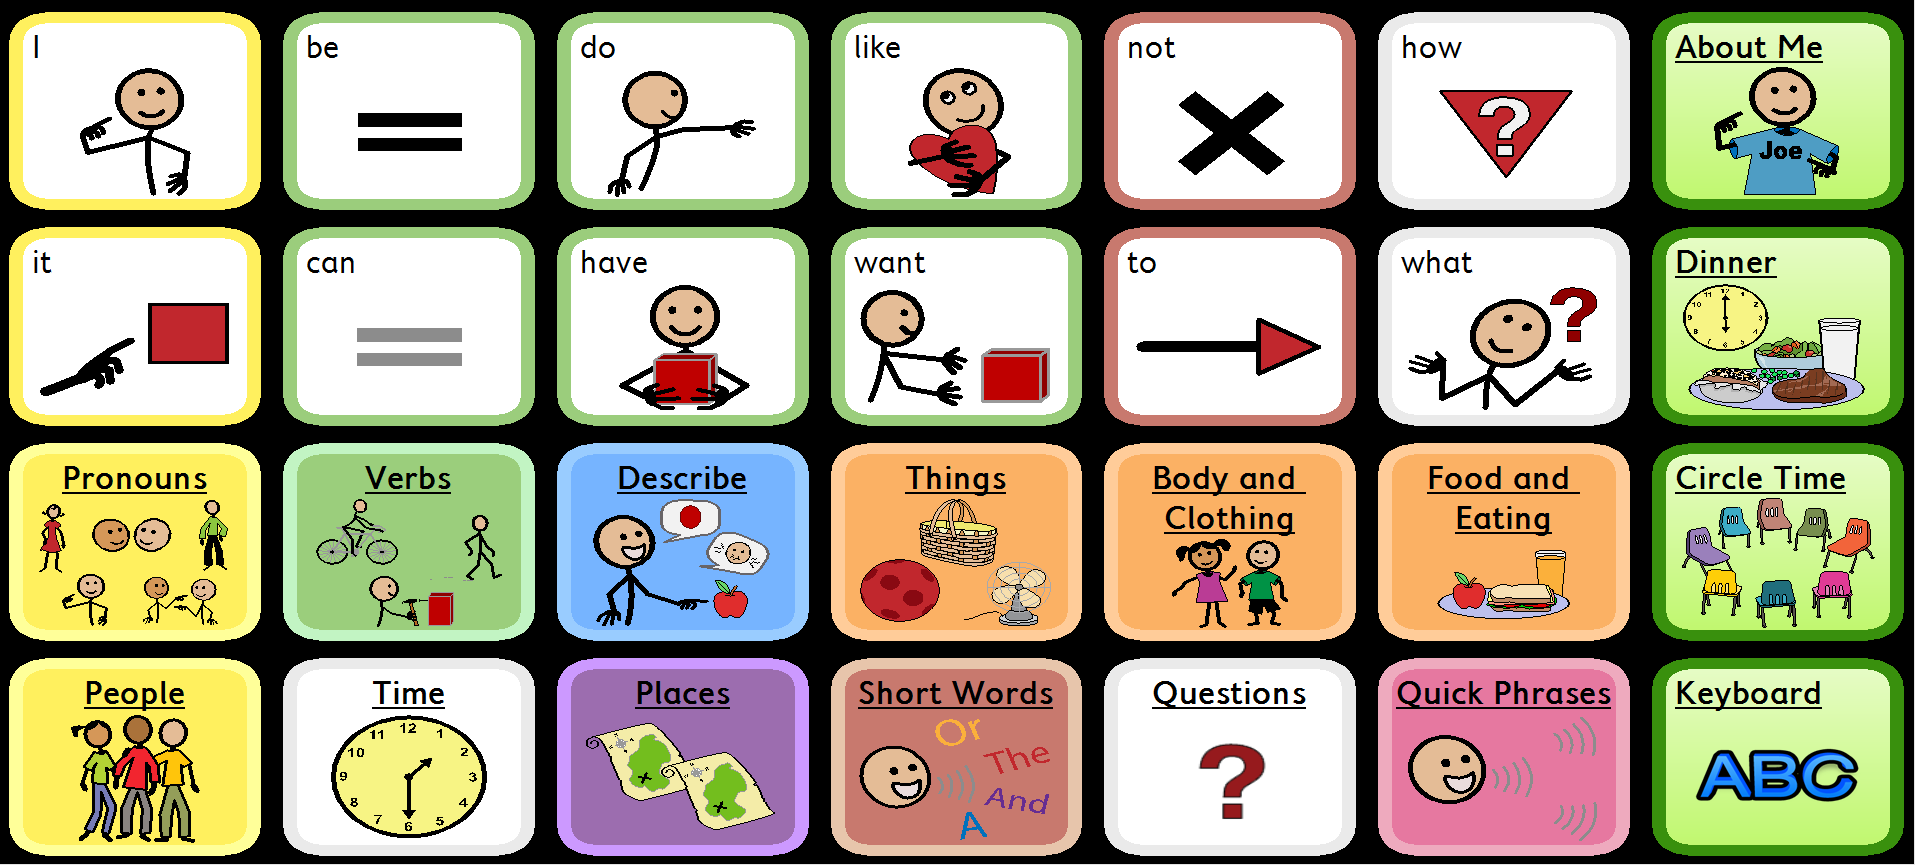
\includegraphics[width=100mm]{symbolgrid}
\caption{Symboltabellen til programvaren Sono Flex}
\label{fig:symbolgrid}
\end{figure}


\section{Kommunikasjonsform: Symboler}

De som ikke har mulighet til å bruke skrift som kommunikasjonsform kan bruke tegnsystemer. Det eksisterer tre typer tegnsystemer: håndtegn (manuelle tegn) som innebærer å bruke håndbevegelser. Materielle tegn, som vil si at en bruker fysiske objekter som brikker eller figurer. Til slutt, grafiske tegn som innebærer at en bruker symboler. 

I denne rapporten vil symbol bli brukt som kommunikasjonsform. Her representerer symboler et ord, frase, uttrykk eller setning. 

Ifølge ISAAC \cite{Tegnsystemer} er grafiske tegn brukt av mennesker med store bevegelsesvansker.
Disse menneskene har utfordringer med å lage manuelle tegn og har forståelsesvansker som følge av lærehemming. Det eksisterer flere pakker med symboler som en kan bruke for å visualisere ord \cite{GrafiskTegn}. I Sono Flex brukes en pakke kalt SymbolStix. I figur \ref{fig:katt} kan du se et eksempel på et symbol. 





\begin{figure}[ht!]
\centering

\includegraphics[width=50mm]{katt}
\caption{Symbol fra pakken SymbolStix}
\label{fig:katt}
\end{figure}

\section{Interaksjonsform: Øyesporing}

Menneske-maskin-interaksjon fungerer ved at en person gir maskinen en kommando, og maskinen svarer med en respons. For at et menneske skal kunne gi en maskin ordre, er det nødvendig at maskinen har en inputenhet som tolker beskjedene fra brukeren, slik at at datamaskinen forstår dem.  Som regel er dette tradisjonelle enheter som tastatur og mus. Det eksisterer derimot mangfoldige måter å samhandle med en maskin på.

I denne rapporten vil brukerinput bli gitt ved en øyesporingsenhet. Ved å fange opp brukerens skuepunkt med et videokamera og infrarøde lys, er det mulig for maskinen å beregne hvor på monitoren personen ser. Dette gjør interaksjon mellom dem mulig. En knapp vil for eksempel bli aktivisert ved at brukeren ser på den en viss periode. Øyesporing vil bli diskutert i neste kapittel.

\subsection{Brukerinteraksjon}

Sono Flex tilbyr to måter for brukerinteraksjon, mus og øyestyring. Mus fungerer som vanlig ved at brukeren svever med musepekeren over ønsket knapp og venstreklikker for å aktivere. Ved øyestyring må brukeren fokusere blikket på ønsket knapp en gitt tid for at applikasjonen skal tolke det som et klikk. 

Det som skjer er at med engang brukeren fokuserer blikket på en knapp vil en nedtelling starte. Figur \ref{fig:knapp-interaksjon} viser hvordan brukeren presenteres for hvor mye av nedtellingen som gjenstår.  Hvis brukeren ikke flytter blikket før nedtellingen har nådd null, tolkes dette som et klikk.
For å gi brukeren beskjed om et godkjent klikk, dannes det en rød firkant rundt knappen. 

\begin{figure}[ht!]
\centering
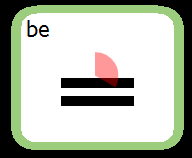
\includegraphics[width=50mm]{Knapp-interaksjon}
\caption{Skjermdump som viser hvordan nedtellingen på en knapp ser ut. Når den røde sirkelen er komplett oppfattes det som et klikk}
\label{fig:knapp-interaksjon}
\end{figure}


\section{Organisasjon og Navigasjon}

Som nevnt i seksjon \ref{subsec:navigasjon} vil et barns vokabular være såpass stort at en nødvendigvis må fordele ordene over flere sider. Sono Flex har eksempelvis 106 ord under kategorien "Ting". Med tanke på at det maksimalt er plass til 28 ord på hver side, må disse fordeles og det må finnes en måte å navigere mellom sidene på. Løsningen har blitt en svært flat struktur med et hierarki på maksimalt 2 nivåer, ergo det finnes ikke underkategorier. 

Figur \ref{fig:hieraki-ting} viser hvordan dette fungerer i praksis. Når man trykker på kategorien "ting", fylles tabellen med 27 ord som passer inn i kategorien "ting". Hvis man ikke finner ønsket ord på den første siden, navigerer man videre med knappen "neste side" og ordene i tabellen erstattes av nye ord. 


\begin{figure}[ht!]
\centering
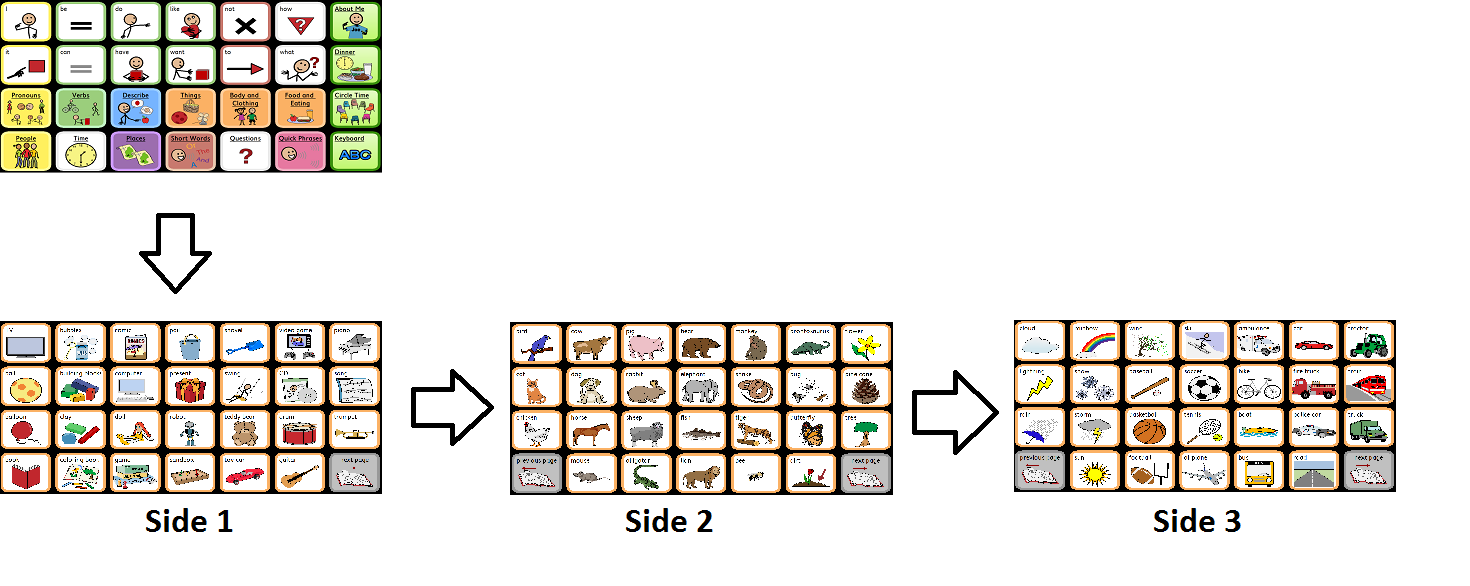
\includegraphics[width=140mm]{Symbgrid}
\caption{Skjermdump hierakiet til Sono Flex}
\label{fig:hieraki-ting}
\end{figure}


\chapter{Øyesporing}

I dette kapittelet blir det gitt enkel forklaring over øyet og hvordan der er mulig å spore det ved hjelp av en øyesporingsenhet. Til slutt vil enheten som brukes i prototype og hvordan den brukes bli presentert.


\section{Hvordan fungerer øyet?}

Å forklare hvordan øyet fungerer i detalj er utenfor denne rapportens omfang. Det vil derimot gitt en enkel forklaring av hvordan det fungerer og de mest nødvendige konseptene.

\subsection{Synsfelt}

I en artikkel skrevet av Tobii \cite{Calibration} sammenlignes øyet med et fotoapparat på grunn av dens mange likhetstrekk. Det hele starter ved at når lys treffer et objekt så reflekteres det. Og på samme måte som et kamera så fanges det reflekterte lyset opp av en linse, som igjen prosjekterer det på en lyssensitiv overflate. Men i motsetning til et kamera er ikke denne overflaten like sensitiv overalt i øyet. Dette gjør at menneske kan tilpasse synet etter hvor mye lys som er tilgjengelig. En bieffekt er at menneske kun kan se klart i begrensede områder av synsfeltet. Dette er illustrert i Figur \ref{fig:visueltArea}, som viser hvordan synsfeltet hos menneske er delt inn etter klarhet. Det innerste området notert ved bokstaven F representerer det foveale området, også kjent som skarpsynet. Dette er den delen av synsfeltet man fokuserer på og som man derfor oppfatter som klarest. Det er hovedsaklig fra dette området visuell data hentes fra. Området deklarert med bokstavene Pf i figuren viser det parafovela området. Som er et overgangsområde og kjennetegnes ved at uskarpheten gradvis øker til man kommer til det perifere området vist som P i figuren. Det perifere området, også kjent som sidesynet, er det mest uskarpe området og fungerer kun bra til å fange opp bevegelser og kontraster.

\begin{figure}[ht!]
\centering
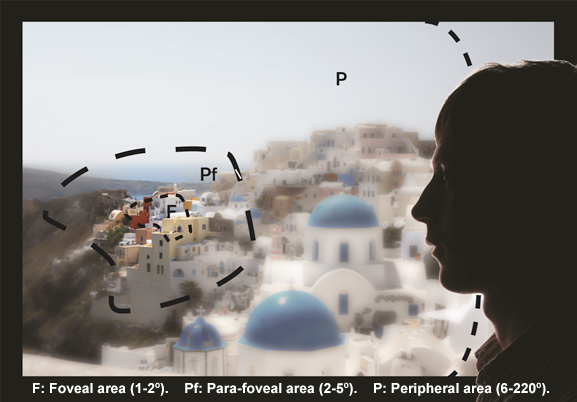
\includegraphics[width=65mm]{fovealArea}
\caption{Bilde/Illustrasjon av menneskelige synsfelt \cite{VisualImage}}
\label{fig:visueltArea}
\end{figure}

\subsection{Øyebevegelser}

Det foveale området er som tidligere nevnt det området det registreres mest visuell data. Ulempen er at området kun står for rundt 2 grader av synsfeltet \cite{Backg0:online}. Så hvis en ønsker å hente detaljert informasjon fra andre deler av synsfeltet, må det foveale området flyttes ved å bevege øyene. De ulike øyebevegelsene som brukes er beskrevet i Listen under er hentet fra nettsiden synstap \cite{sanse7:online}.

\subsubsection{Grovmotoriske}
\begin{itemize}
\item Akkomodasjon – øyets evne til å se klart på forskjellige avstander, det å kunne se skarpt når en flytter blikket hurtig fra avstand til nært og omvendt
\item Følgebevegelser – kunne følge en gjenstand med blikket i alle retninger uten å bevege hodet
\item Konvergens – kunne holde blikket samlet på nært hold
\item Stereosyn – evnen til å se avstand og dybde
\end{itemize}
\subsubsection{Finmotoriske}
\begin{itemize}
\item Sakkader – små forflytninger med blikket ved for eksempel lesing
\item Minisakkader – minibevegelser av øyet (dirring), som må være tilstede for at det skal sendes informasjon til hjernen
\item Antisakkader – evnen til å undertrykke en øyebevegelse
\item Fiksering – evnen til å holde blikket stødig festet på ett punkt
\end{itemize}



\section{Hva er øyesporing?}

Øyesporing er prosessen med å måle hvor en person ser, eller bevegelsen til et øye i forhold til hodet \cite{Eye t4:online}. Ved å gjøre dette kan man finne ut hvilke elementer brukeren ser på, hvor lenge han ser på det og hvordan han beveger blikket. 


\subsection{Bruksområder}

Øyesporing kan anvendes på flere måter. Blant annet så brukte Alfred L. Yarbus øyesporing det til forskning. I sin artikkel fra 1967 \cite{wexle4:online} beskriver han hvordan et subjekts øyebevegelser blir påvirket av oppgaven han skal gjennomføre. Bilde \ref{fig:yarbus} viser hvor forskjellig en person ser på et bilde basert på hvilken oppgave han er tildelt. I tilegg til vitenskap brukes øyesporing også til markedsundersøkelser, reklame, brukervennlighets-testing og mer \cite{Case2:online}. Det som kjennetegner de nevnte bruksområdene er at brukeren ikke aktivt foretar seg noe, han bruker ikke øyene til å gjøre noe annet enn å se. Noe som er annerledes fra anvendelsen i denne oppgaven, hvor øyene i tilegg til å se, brukes til interaksjon.



\begin{figure}[ht!]
\centering
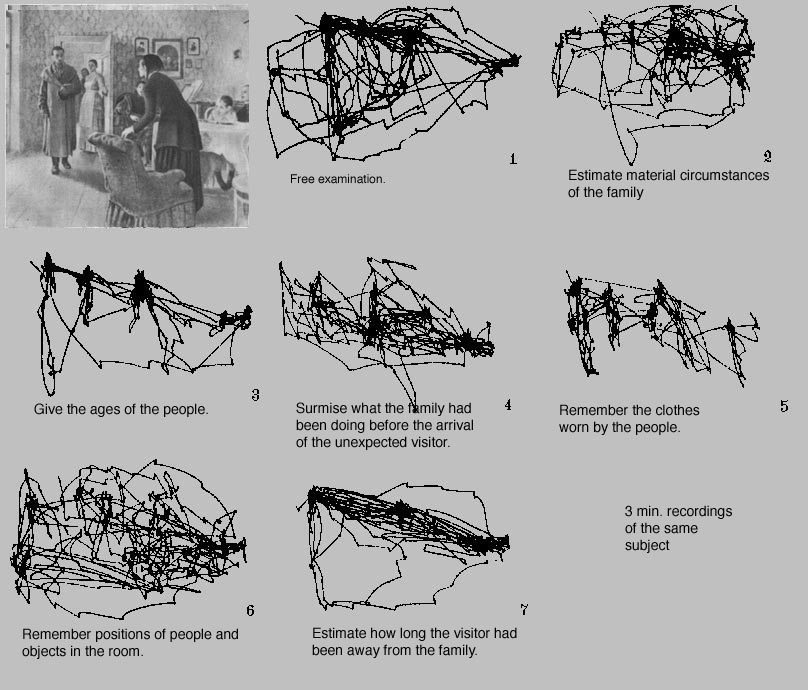
\includegraphics[width=100mm]{Yarbus_The_Visitor}
\caption{Bilde som viser hvordan et subjekts øyebevegelser påvirkes av oppgaven \cite{Yarbu2:online}}
\label{fig:yarbus}
\end{figure}


\subsection{Pupil Centre Cornea Reflection}

Øyesporing er som tidligere nevnt teknikken brukt til å fange og måle øyebevegelser. Det finnes derimot flere fremgangsmåter. I denne oppgaven vil det brukes en ikke-forstyrrende øyesporingsenhet. Dette gjør at brukeren i prinsippet ikke skal legge merke til enheten. For denne typen øyesporing er det mest vanlig å bruke en teknikk som heter Pupil Centre Cornea Reflection (\gls{PCCR}) \cite{Calibration}. Teknikken fungerer ved at en lyskilde belyser øyet for at refleksjonene skal bli klare og synlige. Et kamera tar deretter bilde av refleksjonene fra øyet. Bildet blir så brukt til å identifisere lysets refleksjon på hornhinnen og pupillen. Når en vet vinkelen mellom hornhinnen og pupillen er det mulig å regne ut en vektor. Vektoren sammen med andre geometriske egenskaper ved refleksjonene gjør det mulig å kalkulere ut blikkretningen(Der brukeren ser) \cite{Calibration}.


\section{Tobii PCEye Go}

I prototypen har vi valgt å ta i bruk øyesporingsenheten Tobii PCeye GO \cite{Contr4:online}, som er vist på bilde \ref{fig:tobiiPc}. Enheten kommer separat og kobles til datamaskinen via USB. Denne enheten ble valgt fordi den brukes i Sono Flex og fordi kontaktpersonen i Tobii allerede hadde god erfaring med enheten. Den har også den foredelen at den er av den ikke-forstyrrende typen. Det vil si at en bruker i teorien ikke vil plages av enheten. Noe som hadde vært tilfelle ved å bruke brillene vist på bilde \ref{fig:tobii_glasses} til øyesporing.


\begin{figure}[ht!]
\centering

\includegraphics[width=50mm]{TobiiEyeGo}
\caption{Bilde av øyesporingsenheten Tobii PCEye Go}
\label{fig:tobiiPc}
\end{figure}

\begin{figure}[ht!]
\centering
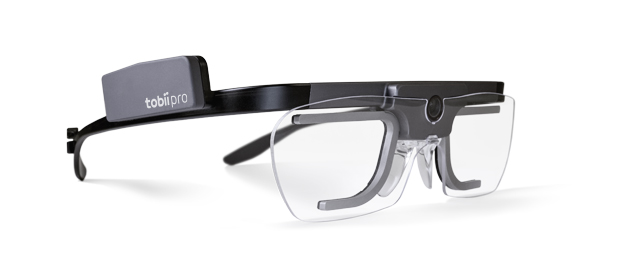
\includegraphics[width=50mm]{Tobii_Glasses}
\caption{Øyesporingsenhet i form av briller som brukeren har på seg}
\label{fig:tobii_glasses}
\end{figure}


\subsection{Tobii Eye Control API }

Figur \ref{fig:overview} viser hvordan blikk interaksjonsserveren eksponerer funksjonalitet til en klient-applikasjon gjennom APIet kalt Tec API. For å ta i bruk TecAPIet tilbys to aksess punkter. Et gjennom .NET plattformen kalt TecClient og et for C dynamisk link library kalt MPACI.  Den praktiske betydningen, er at man kun kan bruke APIet ved å skrive i C eller .NET teknologier. I denne rapporten vil kun sistnevnte være interessant, altså .NET APIet kalt TecClient.


\begin{figure}[ht!]
\centering
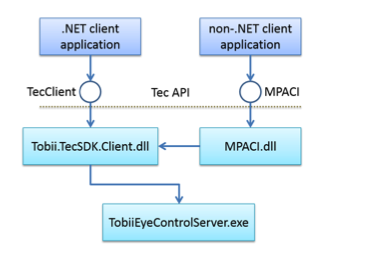
\includegraphics[width=100mm]{SoftwareArchitectureOverview}
\caption{Bilde som viser programvare arkitekturen til blikk programvaren}
\label{fig:overview}
\end{figure}


\subsection{TecClient}

For å gi tilgang til API funksjoner er TecClient komponentet for .NET delt inn i verktøys klasses(toolbox classes). Figur \ref{fig:toolbox} viser de ulike verktøyene som er tilgjengelig. 

\begin{figure}[ht!]
\centering
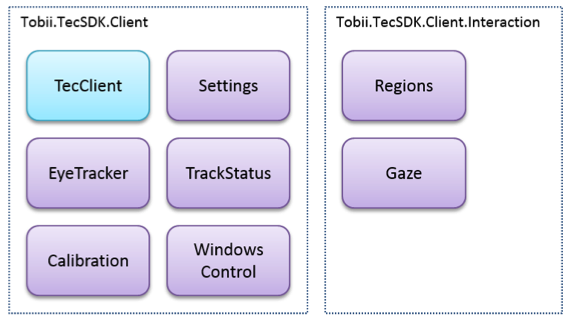
\includegraphics[width=100mm]{Toolbox}
\caption{Verktøy klassser som er tilgjengelige gjennom TecClient komponenten verktøyskasse}
\label{fig:toolbox}
\end{figure}


\textbf{EyeTracker} Gir informasjon om den aktuelle øyesporingsenheten. 

\textbf{Kalibrering} 
For optimal øyesporing med Tobii PCeye Go må enheten kalibreres for hver bruker. Dette verktøyet går gjennom en prosedyre for å måle karakteristikk ved personens øyer som brukes igjen til å lage en fysiologisk 3d modell for å kalkulere hvor brukeren ser \cite{www.t5:online}. Bilde \ref{fig:kalibre} viser et bilde fra kalibreringsprosessen, hvor brukeren blir bedt om å se på de ulike punktene.

\begin{figure}[ht!]
\centering
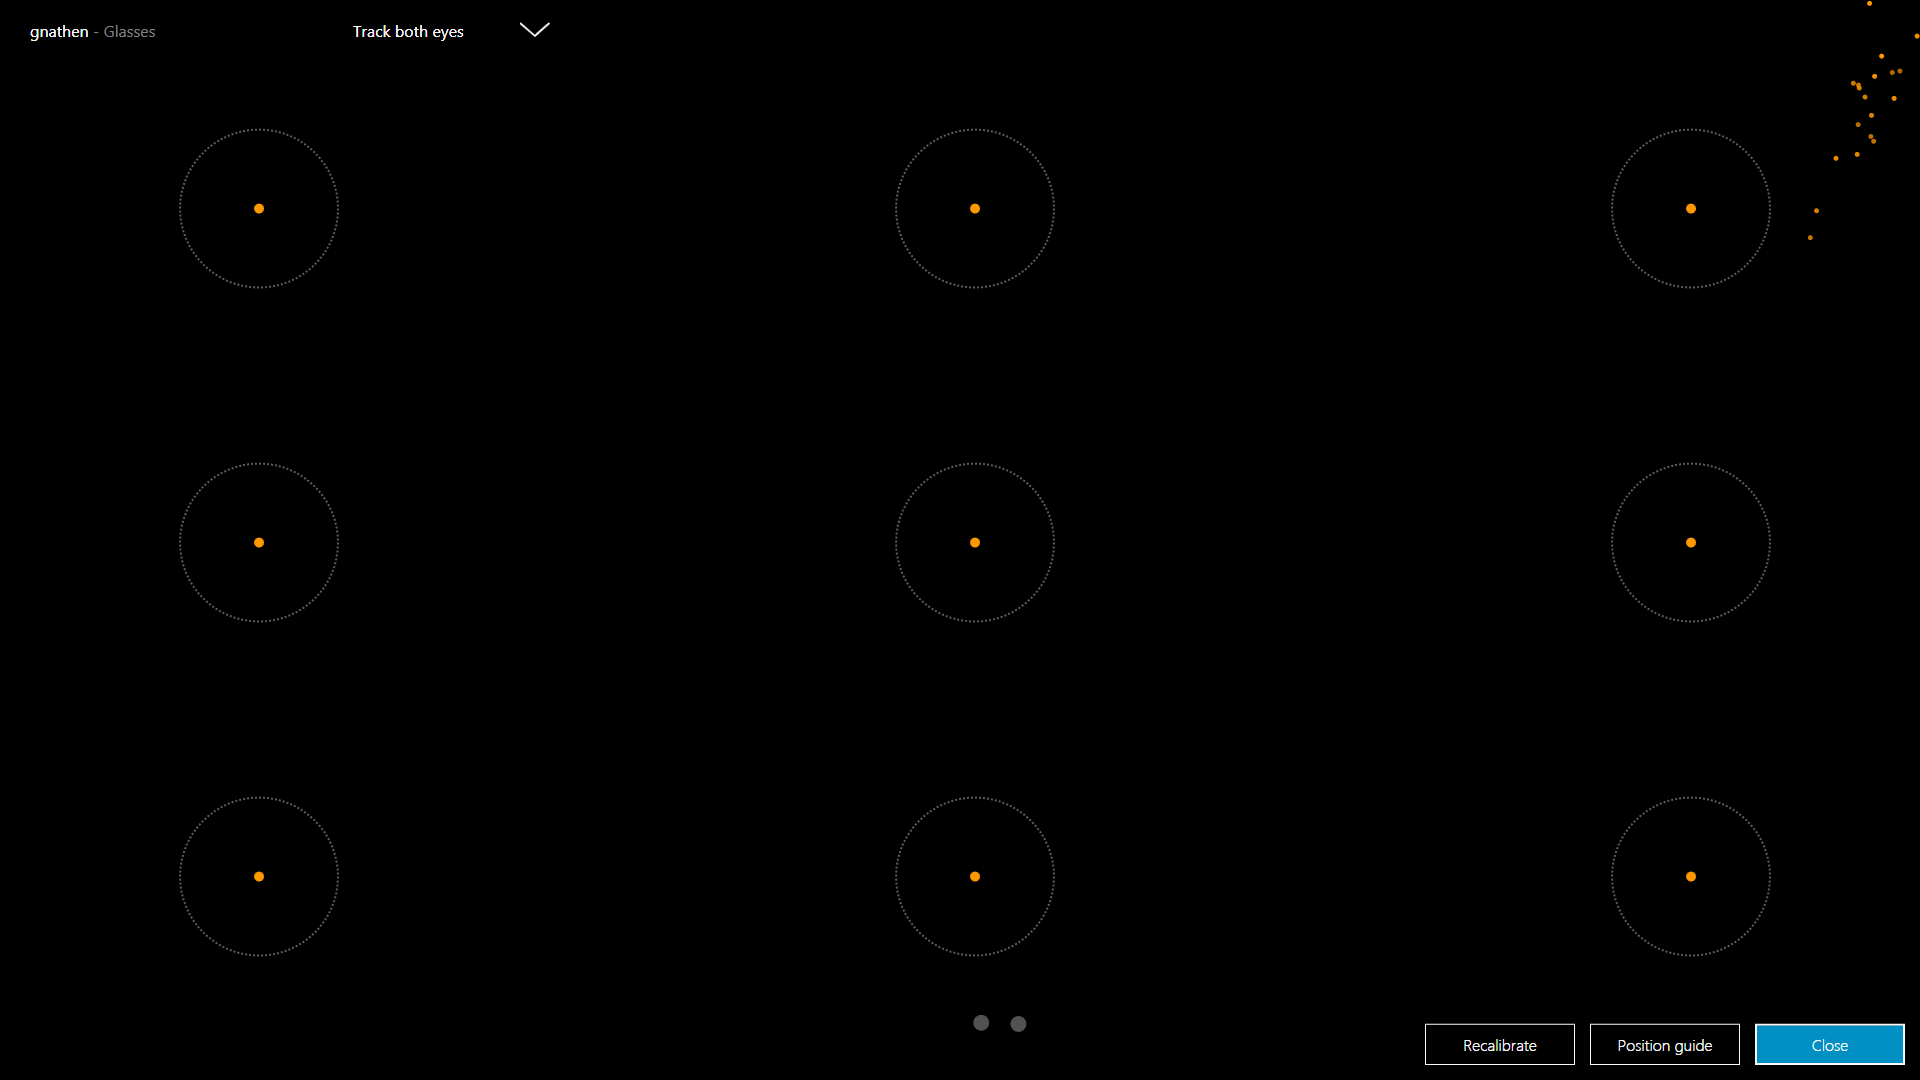
\includegraphics[width=100mm]{kalibrering}
\caption{ \cite{VHye88:online}}
\label{fig:kalibre}
\end{figure}


\subsubsection{Settings}
Settings komponente gir tilgang til brukerprofiler og operasjoner som gjør at man kan skifte mellom dem. For eksempel er det naturlig at en bruker ikke vil gå gjennom kalibreringsprosessen hver gang han vil ta i bruk enheten. I dette komponentet kan karakteristikken fra kalibreringen lagres i brukerprofilen som er er koblet til brukeren, slik at han slipper dette. 


\subsubsection{Trackstatus}
Tilbyr metoder, egenskaper og hendelser for å kontrollere sporingsstatus vinduet. Bilde \ref{fig:track} viser hvordan dette komponentet kan brukes til å vise brukeren om enheten fanger opp øyene og hvordan de er iforhold.

\begin{figure}[ht!]
\centering
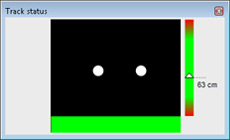
\includegraphics[width=100mm]{Trackstatus}
\caption{}
\label{fig:track}
\end{figure}

\subsubsection{Gaze}
Eksponerer rå blikkdata, både filtrert og ufiltrert. Det vil si at man kan kan finne ut hvor på skjermen en bruker ser i form av X og Y koordinater.


\subsubsection{Region / Interaction regions}

Ifølge dokumentasjonen er en interaksjon region er en geometrisk region på skjermen som en bruker kan interagere ved å se på den (dokumentasjon). En knapp i applikasjon vil typisk bli definert som en interaksjon region. Ved å definere en region kan man lytte til hendelser fra dem. De to viktigste hendelsene er \textbf{Focus} og \textbf{Activation}. Focus hendelsen vil aktiveres når en bruker skuer innenfor grensene til en region. En bruker vil bli opplyst om at han er innenfor en slik region ved hjelp av en indikator. Denne indikatoren vil typisk gi brukeren et signal om at en nedtelling har startet. Når nedtelling er ferdig vil Activation hendelsen bli avfyrt. Activation er konseptuelt det samme som å klikke med en datamus, og responsen vil normalt være den samme.





\chapter{Prototypen} 

I dette kapittelet vil det bli gitt en innføring i valg som ble tatt før og underveis i utviklingen av prototypen. 
 
\section{Utgangspunkt} 
\label{sec:utgangspunkt} 

Målet med oppgaven var å undersøke potensielle forbedringer som kunne implementeres i programvaren Sono Flex. Det mest naturlige valget ville da  ha vært å utviklet de ønskede endringene i den eksisterende koden. Tobii Dynavox ville derimot at de skulle implementeres på en annen plattform. Den ene grunnen var at den eksisterende teknologien hadde flere begrensninger som ville gjort det vanskelig å fått implementert mye av funksjonalitet som skulle undersøkes. Spesielt gjelder dette animasjonene. Den andre var at Windows Forms, som Sono Flex er bygget på,  er satt til å  kun vedlikeholdes av Microsoft  \cite{AAAWPF8:online}.  Det vil si at bugs og feil blir fikset, men at ingen nye funksjoner vil bli lagt til. Dette kan også tyde på at den utfases og at de har valgt å fokusere utviklingen på en annen teknologi. Tobii var derfor interessert i å finne en annen plattform å bygge programvaren på.

Utviklingen startet derfor som et nytt prosjekt og at første del ble å lage en high-fidelity prototype ved å bruke "reverse engineering" på Sono Flex. Det vil si at funksjonaliteten og det meste av utseende skulle være det samme, men at implementasjonen og teknologien ville bli annerledes.


\section{Kravspesifikasjon} 


Å utvikle all funksjonaliteten som Sono Flex tilbyr ville vært for ressurskrevende og derfor utfor denne oppgavens omfang. Det ble derfor bestemt å kun fokusere på det mest nødvendige og heller opprettholde god kodekvalitet. For å finne ut hva som var mest nødvendig og av interesse ble det i samtaler med Tobii funnet en del krav og funksjoner som de ønsket. Disse er spesifisert i listen under og er sortert etter prioritering. 
 
\subsection{Funksjonelle krav} 
 
\textbf{Bygge setninger} – En bruker skal ha mulighet til å sette sammen enkle setninger. Helst skal kompleksiteten til  en setningen begrenses av brukerens vokabular og ikke av systemets mangler.
 
\textbf{Øyesporing som interaksjon} - Det skal være mulig å operere prototypen ved å \underline{kun} bruke øynene. En som tar i bruk øyesporing skal ha tilgang  på samme funksjonaliteten som hvis han hadde tatt i bruk datamus. Det skal også jobbes for å få effektiviteten så lik som mulig mellom de to interaksjonsformene. 
 
\textbf{Bilde for vært ord} - For vært ord skal det være en billedlig fremstilling av det. En bruker, skal i teorien, kun ved å se på bildet forstå hvilket ord det representerer. 

\textbf{Norsk} – Det skal være støtte for norsk. Ord og all tekst skal være på norsk.
Det bør også legges opp til at en enkelt kan skifte språk. 

\textbf{Tale} - Systemet skal kunne gjøre setninger som brukeren har skrevet om til lyd. Jo mer naturlig talen høres ut jo bedre.
  
\textbf{Brukertilpasning} - Hver bruker skal ha mulighet til å kunne tilpasse programvaren etter sine preferanser.
  
\textbf{Animasjon og Lydeffekter } - I prototypen skal en bruker ha mulighet til å aktivere animasjoner og lydeffekter. Disse skal bli avspilt når en bruker trykker på de ulike symbolene.  Neste kapittel vil spesifisere dette i detalj.

\textbf{Logging} - I systemet skal det være mulig å kunne logge all interaksjonen en bruker gjør med programvaren. Denne funksjonen vil være nødvendig for å kunne gjennomføre testingen 

\subsection{Ikke-funksjonelle krav} 
 
\textbf{Kodekvalitet} - Kodebasen skal være tilrettelagt for vedlikehold og videreutvikling. En viktig del av oppgaven var at personer som ikke har deltatt i systemutvikling skal ha mulighet til å forstå koden slik at de enkelt kan legge til og fikse funksjoner. Programvaren skal også legge opp til at det er enkelt og bytte ut animasjoner, lyd og nye symboler. 

\textbf{Brukervennlighet} - Målgruppen består av barn som har begrenset erfaring med å operere dataprogrammer. Det er derfor viktig at det legges vekt på dette og at programvaren utformes på en måte som er intuitiv for brukeren.   
 
 \textbf{Responstid} -  Programvaren er kompleks og det tar lang tid å skrive med symboler, det er derfor viktig at systemet responderer kjapt og ikke gjør at oppgaven tar lenger tid enn nødvendig. Når brukeren trykker på noe skal det føles som om programvaren svarer momentant. 

\textbf{Personvern} - Brukerne av programvaren er en sårbar gruppe, det vil derfor være viktig at sensitiv informasjon ikke kommer på avveie. Det skal i utgangspunktet ikke lagres sensitiv data, men hvis data lagres skal det lagres på en sikker måte. 
 
\section{Utvikling} 
I denne seksjonen vil teknologier og arbeidsområde bli beskrevet.  
 
\section{Programmeringsrammeverk} 

Et programmeringsrammeverk var ikke nødvendig for å kunne bygge prototypen, men har flere fordeler som gjorde at det ikke kunne utelates. Blant det viktigste er lav-nivå kode som allerede har blitt testet og brukt av andre programmerere \cite{Frame7:online}. Dette øker påliteligheten til koden og reduserer utviklingstiden.
Til å utvikle prototypen ble programmeringsrammeverket .NET brukt. Dette ble valgt på grunn av at dokumentasjonen til øyesporingsenheten anbefaler det og alle eksemplene i dokumentasjonen bruker det. En annen grunn var at dette rammeverket tilbyr flere gode brukergrensesnitt-teknologier som var ønskelig med tanke på at prototypen som skulle utvikles var svært grafisk.

\subsection{.NET}
 
Som en kan se på figur \ref{fig:net-arkitektur}  er arkitekturen til .NET omfattende og har flere programmeringsspråk og komponenter en kan velge å ta i bruk. Rapporten vil kun gi informasjon om de ulike komponentene fra .NET som ble brukt eller som er nødvendig for forståelse av valgene som har blitt tatt. 
 
 
\begin{figure}[ht] 
\centering 
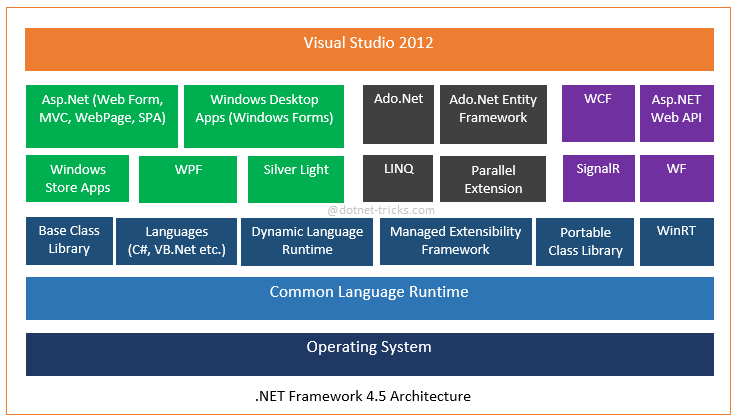
\includegraphics[width=140mm]{netframework45} 
\caption{Diagram som viser arkitekturen til .net rammeverket versjon 4.5} 
\label{fig:net-arkitektur} 
\end{figure} 
 
 
\section{Brukergrensesnitt-teknologi} 

Brukergrensesnitt-teknologi gir utvikleren tilgang på funksjoner og forhåndsdefinerte grafiske elementer som skal gjør utviklingen mer effektiv. Som en kan se ut ifra figur \ref{fig:net-arkitektur} tilbyr .NET teknologier som Windows Store Apps, Windows Presentation Foundation(\gls{WPF}), Windows Forms og Silverlight. Alle disse ble evaluert før et endelig valg ble foretatt:

\textbf{Windows Forms} ble utelukket ettersom dette er teknologien som Sono Flex er bygget på og som hadde begrensinger som gjorde at flere av de ønskede funksjonene ble vanskelig å implementere. 

\textbf{Windows Store Apps} hadde mye av den ønskede funksjonaliteten, samtidig som den fortsatt vedlikeholdes. Problemet var at for å distribuere slike applikasjoner brukes Windows Store og for å få publisert applikasjonen der, kreves godkjenning av Windows. Dette i sammenheng med at disse applikasjonene ikke er kompatible med Windows 7\cite{Windo0:online} gjorde at denne teknologien ikke ble valgt. 

\textbf{Silverlight} er ifølge Microsoft sin blogg\cite{User1111:online} en kraftig utviklingsplattform for å lage "rike" media- og forretningsapplikasjoner for web, skrivebord og mobil. Fokuset til teknologien er derimot på web og mobil \cite{Micro6:online}, og ettersom prototypen er en skrivebords applikasjon falt ikke valget på Silverlight.

Teknologien som til slutt ble valgt var \textbf{Windows Presentation Foundation}. WPF skal tilby utviklere en helhetlig programmeringsmodell for å bygge skrivebords applikasjoner for Windows som tar i brukergrensesnitt, media og dokumenter \cite{Windo777:online}. Grunnen til at teknologien ble valgt er:


\begin{itemize}
\item Fokus på skrivebord. I motsetning til blant annet Silverlight, er WPF designet og laget for å utvikle klient applikasjoner\cite{Windo777:online}.
\item Prioritert av Tobii PC Eye GO. I dokumentasjonen til øyesporingsenheten er det skrevet: "WPF  rammeverket er et svært bra verktøy for utvikling av grafikk-intensive applikasjoner og WPF har derfor blitt gitt høyest prioritet [..]"
\item Etterfølgeren til Windows Forms . WPF er ifølge Microsoft erstatteren til teknologien som blir brukt i Sono Flex \cite{User1111:online}. 
\item God støtte for animasjoner. WPF tilbyr blant annet et eget timing system for å enkelt holde tiden når en animerer grafiske elementer \cite{Anima7:online}.
\end{itemize}



 
\subsection{Windows Presentation Foundation} 
 
Ifølge Adam Nathan \cite[p.~9]{WPFbook}, programvare arkitekt hos Microsoft, ble prosessen med å lage WPF igangsatt fordi ingen hadde adressert vanskeligheten med å lage moderne brukergrensesnitt. Spesielt med tanke på at grafisk maskinvare hele tiden har blitt bedre og billigere sammen med at forbrukernes forventninger har fortsatt å stige. 
Han argumenterer med at det fantes utviklere på tiden som for eksempel brukte bitmap bilder for å endre utseende på standardknappene. Problemet er at disse formene for tilpasning ikke bare kan være ressurskrevende å utvikle, men også gi en dårligere brukeropplevelse. Han forteller videre at de ønsket å lage et rammeverk som hadde produktiviteten som folk likte med Windows Forms og som var like enkel som HTML og Javascript.

WPF gir utvikleren mulighet til å utvikle applikasjoner med både markup- og programmeringspråk. Markup språket brukes vanligvis til å implementere utseende til applikasjonen, mens programmeringsspråket brukes vanligvis til å implementere oppførselen. Det vil si at det er mulig å bruke de på tvers, men WPF legger opp til å skille mellom utseende og oppførsel \cite{Intro8:online}. Dette skillet skal ifølge utviklerne gi flere fordeler som blant annet reduksjon av utvikling- og vedlikeholdskostnader. Fordi utseende-spesifikk markup ikke er tett koblet med oppførsel-spesifikk kode. Skillet mellom dem gir også designere mulighet til å jobbe med utseende samtidig som utviklere jobber med oppførsel \cite{Intro8:online}. I WPF er eXtensible Application Markup Language (XAML) brukt som markup språk. Mens man som programmeringsspråk kan velge mellom C-Sharp eller Visual Basic.

\subsubsection{C-Sharp} 

Valget av programmeringsspråk sto mellom C-Sharp og Visual Basic (VB), to språk med svært forskjellig syntaks og historie \cite{Compa6:online}. C-Sharp har basert syntaksen sin på programmeringsspråket C , mens VB har sine røtter fra programmeringsspråket BASIC \cite{Visua3:online} \cite{About8:online}. Begge språkene har de samme mulighetene, forskjellen ligger hovedsakelig i syntaks, så valget av programmeringsspråk ble basert på preferanser \cite{What0:online}. I dette tilfelle ble det valgt å ta i bruk C-Sharp, mest på grunn av likheten med Java som vi hadde erfaring med fra tidligere.


\subsubsection{eXtensible Application Markup Language (XAML)} 

XAML, en dialekt av XML, har vært en viktig del av WPF siden dens introduksjonen i 2006 \cite[p.~17]{WPFbook}. Vanligvis brukes XAML til å spesifisere brukergrensesnitt objekter og organiseringen av dem, men kan også brukes til andre ting som for eksempel animasjoner \cite{Story5:online}. 

Grunnen til at XAML har blitt brukt er fordi det er enkelt for programmere å samarbeide med eksperter fra andre felt. Nathan forteller at XAML blir fellesspråket for alle partiene, hovedsakelig gjennom utviklingsverktøy og felt-spesifikke design verktøy. Men også fordi XAML (og XML generelt) er enkelt å lese og forstå \cite[p.~17]{WPFbook}. Figur \ref{listing:knapp} viser hvor enkelt en kan genere en blå knapp som også er lettleselig .


\begin{listing}[ht] 
\inputminted[fontsize=\footnotesize, frame=lines,framesep=2mm,baselinestretch=1.2,bgcolor=lightgray,linenos]{xml}{Code/xamlexample.xml} 
\caption{Hvordan en blå knapp blir definert i XAML} 
\label{listing:knapp} 
\end{listing} 
 
   
\section{IDE og versjonskontroll} 

For å automatisere mye av utviklingen ble det valgt å bruke utviklingsmiljøet Visual Studio 2013 \cite{2013-1:online}. Grunnen til at Visual Studio ble valgt er det fordi den i tillegg til å ha et kode-redigeringsverktøy og debugger, så har den også en WPF designer\cite{What8:online}. Denne designeren tilbyr flere hjelpemidler for å effektivisere prosessen med å lage brukergrensesnitt. Blant annet kan man velge mellom å manuelt skrive grafiske elementer i XAML eller man kan trekke inn forhåndsdefinerte elementer fra et sidepanel. Den viktigste funksjonen som tilbys er derimot design vinduet. Dette viser til enhver tid hvordan brukergrensesnitt blir uten å måtte kjøre koden\cite{WPF D1:online}. 
 
For versjonskontroll ble det av erfaringsmessige årsaker brukt git\cite{AboutGit:online}. Til å ta backup av prosjektet ble den web-baserte tjenesten Bitbucket brukt. Grunnen til dette var at mye av koden fra Tobii Dynavox var konfidensiell og Bitbucket tilbyr hemmelig oppbevaring gratis. 
 
 
\section{Model View ViewModel} 

En viktig del av oppgaven var å utvikle en prototype som Tobii Dynavox kunne bygge og teste videre på. Det var derfor en forutsetning at kildekoden var tilrettelagt for vedlikehold og videreutvikling. Et tiltak som ble gjort for å gjennomføre dette var å følge arkitekt mønsteret Model view Viewmodel (MVVM). Grunnen til at vi valgte dette fremfor mønster som for eksempel Model View Contoller(MVC)\{MVC a2:online} og Model-View-Presenter(MVP)/cite{The M4:online}. Er fordi MVVM ble utviklet av Microsoft spesifikk for å utnytte funksjonaliteten til WPF  og at mønsteret er som skreddersydd for teknologien \cite{THEM6:online}. 

Det ble tidligere nevnt a WPF legger opp til å skille mellom utseende og oppførsel, MVVM skal hjelpe utviklere å følge dette prinsippet. Ved å skille mellom applikasjons logikk og brukergrensesnitt skal det ifølge Microsoft \cite{Im1online}, være enklere å teste, vedlikeholde og videreutvikle. MVVM gjør dette ved å dele opp koden i 3 deler - Modeller, ViewModel og View. Figur \ref{fig:mvvm} viser de tre MVVM klassene view, view-model og model, og interaksjonen mellom disse.
 
\begin{figure}[ht!] 
\centering 
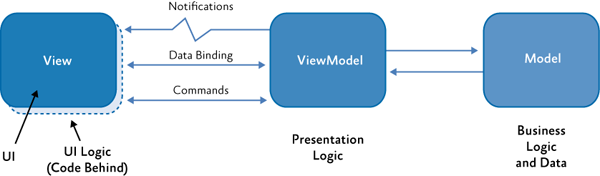
\includegraphics[width=100mm]{Mvvm} 
\caption{Illustrasjon som viser tre MVVM klasser og hvordan interaksjonen mellom dem\cite{Im1online}} 
\label{fig:mvvm} 
\end{figure}


\subsection{Model}

\textit{Model} delen av MVVM står for en av de viktigste delene i enhver applikasjon, nemlig data og informasjon. \textit{Model} sin eneste jobb er å representere og holde dataene som applikasjonen skal bruke. Den skal ikke hente data fra en database eller manipulere data på noen som helst måte \cite{Model7:online}. Dette går under forretningslogikk og skal ifølge mønsteret holdes separat fra model-klasser. 


\subsection{View}
 
 Som navnet impliserer, skal klasser definert som \textit{View} stå for visuelle elementer som vinduer, knapper, tekst, farger og organiseringen av dem. Med andre ord, selve brukergrensesnittet \cite{THEM6:online}. View-klasser vil bli skrevet i XAML.

 
\subsection{ViewModel}
 
 Som en kan se utfra figur \ref{fig:mvvm} ligger \textit{Viewmodel} mellom \textit{Model} og \textit{View}. Så mens \textit{model} holder data og \textit{View} presenterer data så er det \textit{Viewmodel} sin jobb å manipulere og håndtere data. Si for eksempel at \textit{Model} holder en dato lagret i et format som ikke er så lettleselig. Det er da \textit{ViewModel} sin jobb å konvertere det til et mer leselig format før \textit{View} presenterer det til leseren. 
 
\subsection{Databinding, Notifikasjon og Kommando}

Et \textit{View} og en \textit{ViewModel} skal ifølge mønsteret ha en en-til-en relasjon, der \textit{view} har en referanse til \textit{ViewModel}, men ikke omvendt. For at \textit{ViewModel} og et \textit{View} skal kunne "snakke" sammen og fortsatt holdes separat brukes databinding, kommandoer og notifikasjoner. 

\textit{View} presenterer informasjon til brukeren ved å binde seg til egenskaper og kommandoer som \textit{Viewmodel} eksponerer, dette kalles for \textbf{databinding}. Når en egenskap endres i \textit{ViewModel} vil \textit{View} bli oppmerksom på dette gjennom en notifikasjon og oppdateres deretter. 

En kommando er implementert i \textit{ViewModel}, men blir aktivert fra \textit{View}. Dette skjer ved at en bruker trykker på en knapp, \textit{View} klassen vil så forteller \textit{ViewModel} å kjøre en gitt kommando.

\subsection{MVVM-light toolkit} 
 
 MVVM-light er et bibliotek som skal hjelpe utviklere med å sette opp MVVM i kodebasen \cite{Nico0:online}. Hensikt ved biblioteket er å akselerere utviklingen av MVVM applikasjoner i WPF, Silverlight, Windows Store, Windows Phone og Xamarin \cite{MVVM8:online}. Dette skal det gjøre ved å levere et utviklingsklart fundament og flere hjelpeklasser. 


Den viktigste grunnen til at dette tredjeparts biblioteket ble tatt med i prosjektet er på grunn av en funksjon kalt DesignTime-Data \cite{MVVMLightDoc:online}. For en av fordelene ved å skrive brukergrensesnittkode i XAML er at en har mulighet til å se resultatet momentant i et design vindu. Ulempen er at dette kun gjelder for statisk innhold og ikke data som må hentes fra databaser, web-tjenester eller andre kilder. Ved å bruke DesignTime-data kan man bruke en boolsk egenskap som heter IsInDesignModeStatic \cite{MVVM100123:online}. Hvis denne er sann så kan man hente dummy data, hvis ikke så kan det hentes fra den faktiske kilden. Dette gjør at man slipper å kjøre programmet for å se endringer. 


\section{Dataformat og lagring}


Programvaren skal strebe etter å kunne tilby de ordene en bruker har lyst å bruke. En ganske stor utfordring med tanke på at et barns vokabular allerede i alder av 5 år kan være opp i mot 2000 ord. Spesielt med tanke på at hvilket ord dette er, vil variere fra person til person. For vært ord må det også være et symbol som representerer det. En naiv fremgangsmåte ville vært å statisk gjengi hver brikke med et ord og bilde. Problemet med dette er først og fremst at XAML koden blir svært lang, som følge av at en må skrive en knapp for vært tilfelle. Den andre er at en også må inn i koden for å gjøre endringer eller legge til nye ord. 

Løsningen på ble å oppbevare alle ordene i en separat fil for å skille mellom brukergrensesnitt og data. Det ble laget to variasjoner for lagre data - den ene i JavaScript Object Notation(JSON) dokument den andre som et tekstdokument.

\subsection{JSON}

JSON er et lettvekt data-utvekslings format som er lett for mennesker å lese og skrive, og som er lett for maskiner å tolke og generere\cite{JSON7:online}. Figur \ref{listing:jsonfile} viser et utdrag fra en av JSON filene som brukes i prototypen. Hver JSON fil består av en liste med JSON objekter som har attributtene \textit{Name} og \textit{Image}. Der \textit{Name} er ordet og \textit{Image} er stien til et bilde som representerer ordet. Dette er bare et lite utdrag fra filen og viser kun det som ville tilsvart fire brikker i programvaren.

I dette dokumentet er det første objektet "I" et ord, mens de tre neste er kategorier. Hver kategori består av flere ord. Ordene som tilhører en kategori er lagret i en egen fil i en mappe med samme navn. 

Figur \ref{fig:jsonstructure} viser strukturen på filene, der hver kategori har sin egen mappe. Dette gjør at data hentes "just-in-time". Det vil si at istedenfor at ordene ligger i minnet til enhver tid, så hentes de kun når ved behov. Eksempelvis hvis en bruker trykker på kategorien "Food and Drink" så vil ordene hentes fra "FoodAndDrink.json" i mappen "FoodAndDrink". Noe som sparer på minnet, men som kan forringe kjøretiden. For når det er snakk om så store mengder data som alle ordene ville gitt, er det ikke gunstig å bevare dem i minnet. 


\begin{listing}[ht] 
\inputminted[fontsize=\footnotesize, frame=lines,framesep=2mm,baselinestretch=1.2,bgcolor=lightgray,linenos]{json}{Code/JSONfile.json} 
\caption{Utdrag fra filen som inneholder ord og sti til bilde som representerer det i JSON format} 
\label{listing:jsonfile} 
\end{listing} 
 

 \begin{figure}[ht!] 
\centering 
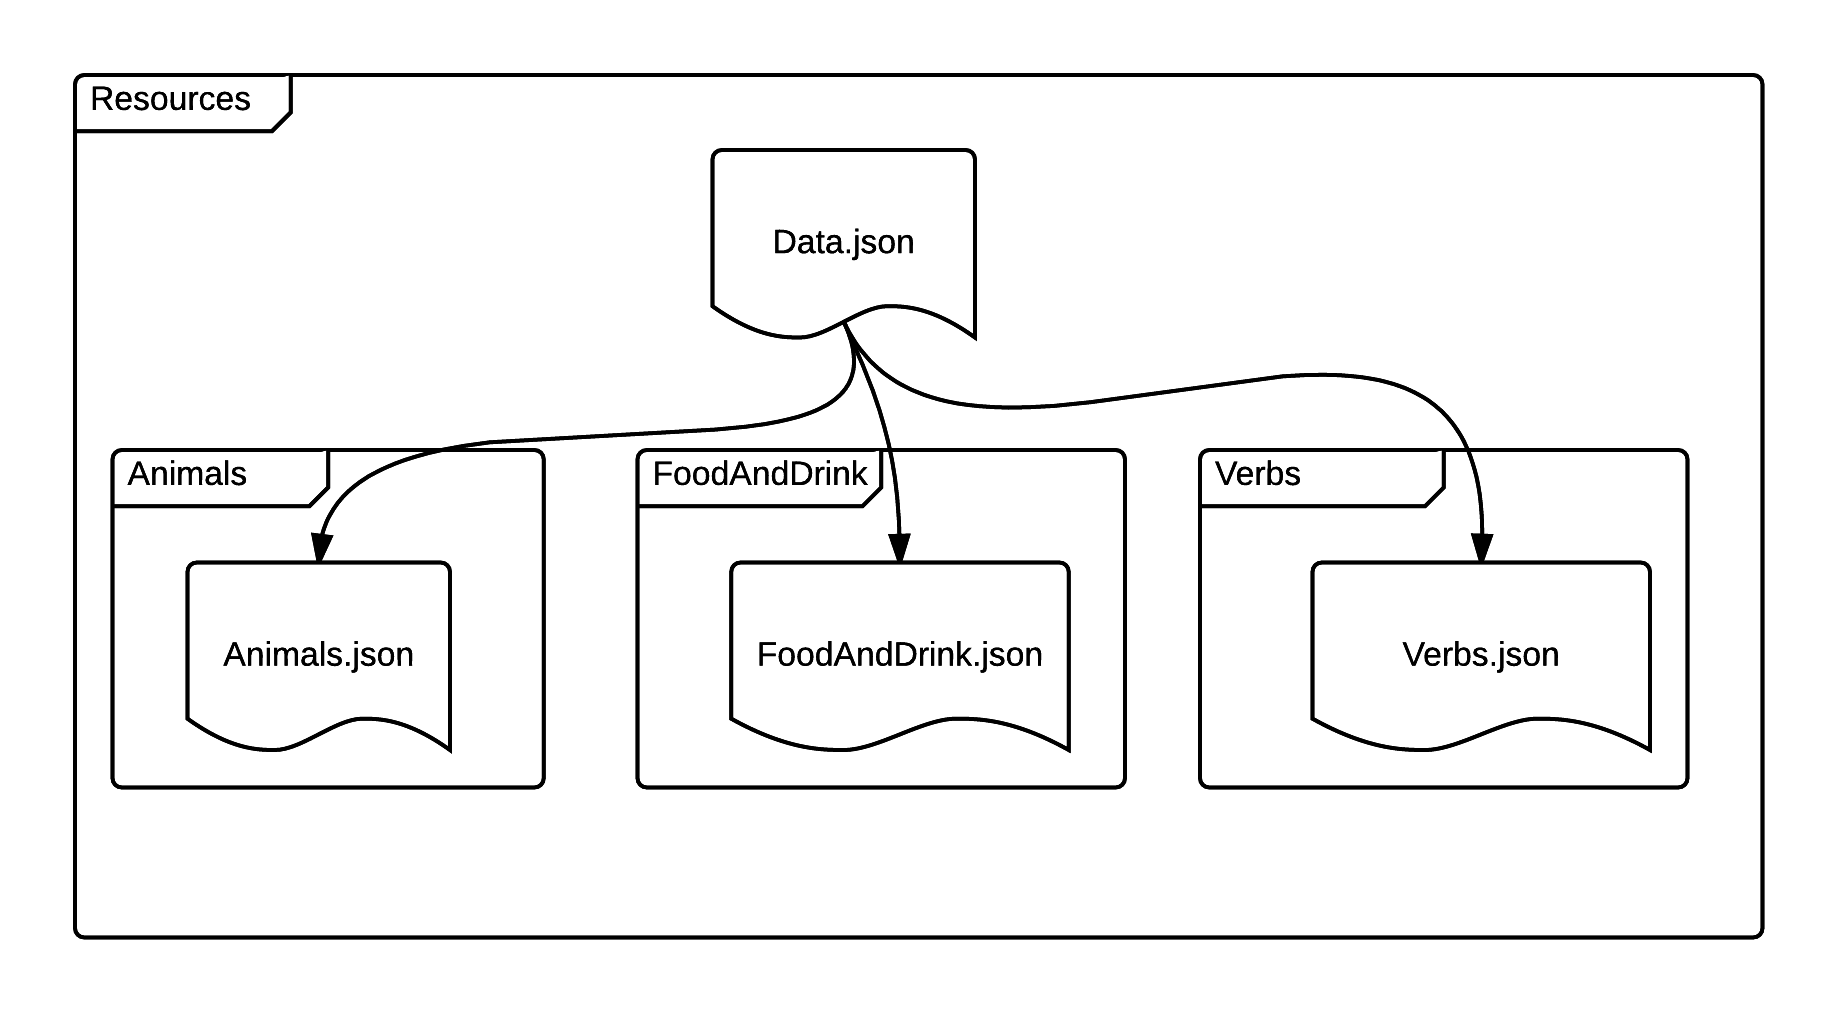
\includegraphics[width=100mm]{JsonStructure} 
\caption{Mappestruktur til et utvalg kategorier} 
\label{fig:jsonstructure} 
\end{figure} 


\subsection{JSON Tolking}

For å kunne ta i bruk objektene definert i tekstfilen må de tolkes om fra JSON format til dataobjekter. Denne prosessen, å trekke ut datastrukturer fra bytes, kalles deserialisering. For å gjøre dette har vi brukt et tredjeparts rammevekt kalt JSON.NET \cite{Json.0:online}. Det finnes en innebygd funksjon i .NET kalt DataContractJsonSerializer \cite{DataC3:online} som også greier å deserialisere et JSON dokument. Grunnen til at JSON.NET ble brukt er fordi i dette biblioteket er det mulighet å automatisk deserialisere en helt liste av JSON objekter til en dataliste uten å manuelt måtte legge inn objektene. Ifølge utviklerens egne nettsider skal rammeverket være 50 prosent kjappere enn DataContractJsonSerializer, men ytelsen er avhengig av hvilke datasett som brukes, og har ikke vært en faktor i avgjørelsen. 


\begin{listing}[ht] 
\inputminted[fontsize=\footnotesize, frame=lines,framesep=2mm,baselinestretch=1.2,bgcolor=lightgray,linenos]{csharp}{Code/JSONparser.cs} 
\caption{Koden som konverterer JSON filen til en Liste} 
\label{listing:JsonParser} 
\end{listing} 


Koden i figur \ref{listing:JsonParser} deserialiserer JSON dokumentet om til en dataliste. Fra linje 5 til 12 skrives teksten fra filen over til en \textit{string}. På linje nummer 14 blir strengen konvertert til et dataobjekt. Dokumentet blir gjort om fra \textit{string} til et komplekst objekt på kun en linje. 


\section{Tekstfil}

Under utviklingen ble det bare lagt inn tilfeldige ord og bilder hentet fra internett i prototypen, men ettersom prototypen begynte å bli ferdigstilt var det behov for et større utvalg ord og symboler. Det ble derfor gitt tillatelse av Tobii Dynavox til å ta i bruk det samme bildene som de bruker i deres programvare. Sammen med bildene fulgte det med et dokument som hadde en beskrivelse av vært bilde og ordet det representerer. For vært ord var egenskapene beskrevet i liste \ref{itm:egenskaper} tilgjengelig. 

\begin{itemize}
\label{itm:egenskaper}
\item Symbol ID
\item Dato oppdatert
\item Dato laget
\item Kategori Navn 
\item Filnavn
\item Filsti
\item Ord
\item Synonymer
\item Tysk, nederlandsk, norsk, svensk, dansk, engelsk, spansk, italiensk, fransk, portugisisk.
\end{itemize}


Hver av egenskapene i listen var separert med et tilde tegn som gjorde at det var mulig å oversette til datastrukturer. I tillegg til å tilby det samme som JSON dokumentet, ord og bildesti, så har den også ordets kategori og synonymer for ordet. Det er også mulighet for å få ordet på flere språk og synonymer til de ulike språkene. Dette åpnet for flere muligheter, men for å få til dette, måtte det legges til en annen form for innlesing av data ettersom dokumentet ikke var lagret i JSON format og i motsetning til å dele opp symbolene opp i separate dokumenter basert på hvilken kategori de tilhørte, så var alle deklarert på et dokument. Så  valget sto mellom å lage et skript som oversatte dokumentet til JSON format eller lage en alternativ innlesning. Å omgjøre det fra tekst til JSON hadde vært mulig, problemet med dette er at dokumentet utsatt for oppdatering fra en ekstern part. Konsekvensen hadde vært athver gang dokumentet ble forandret måtte en ha oversatt det på konvertert det på nytt. Det ble derfor bestemt å heller implementere en teksttolker. 
\subsection{Teksttolker}

Teksttolkeren er mer kompleks enn JSON tolkeren. Hovedsakelig fordi det ikke finnes noe bibliotek som automatisk tilegner egenskaper til symbolene. Egenskapene blir derfor gitt til vært symbol etterhvert som de blir lest inn. En annen utfordring var, som tidligere nevnt, at alt befant seg på et dokument som da totalt utgjorde 16 000 linjer med beskrivelse av symbolene. Slik at hvis en skulle ha brukt samme fremgangsmåte som med JSON parseren å kun lest inn for den gitte kategorien. Så hadde en i verste fall måtte ha lest 16 000 linjer med tekst. Dette er ikke gunstig. Dokumentet har flere kategorier og symboler som ikke er nødvendig for barn, blant annet egne kategorier som eksempel Brasil, hebraisk og sveitsisk. Det ble derfor bestemt å kun velge kategorier som var nødvendige og heller fjerne andre fra dokumentet.

\begin{figure}[ht!] 
\centering 
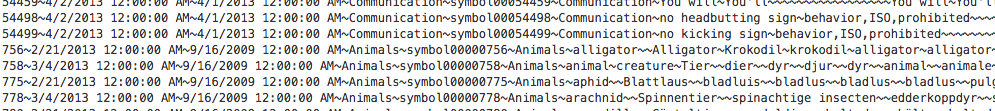
\includegraphics[width=100mm]{datafil} 
\caption{Bilde av dokumentet hvor de ulike symbolene er registrert} 
\label{fig:dok} 
\end{figure} 


\section{Symbol}

Vært objekt i JSON filen og hver linje i tekstfilen blir tolket om til et \textbf{Symbol} objekt. I kontekst av MVVM vil Symbol være en \textit{Model}. Et symbol sine viktigste egenskaper er ordet, stien til bilde som representerer ordet og hvilken kategori ordet tilhører. Den har også egenskaper som synonymer, id, forskjellige språk. Figur \ref{fig:symb} er utdrag fra symboltabellen og viser hvordan 4 symboler ser ut i brukergrensesnittet. De to øverste er ord, mens de to på nederste rad representerer kategorier. Symboler som representerer ord vil alltid ha en hvit bakgrunnsfarge med kategorien den tilhører som kant. Kategorier vil alltid ha en annen enn hvit bakgrunnsfarge. Dette er for at det skal være lettere å skille mellom dem.

 \begin{figure}[ht!] 
\centering 
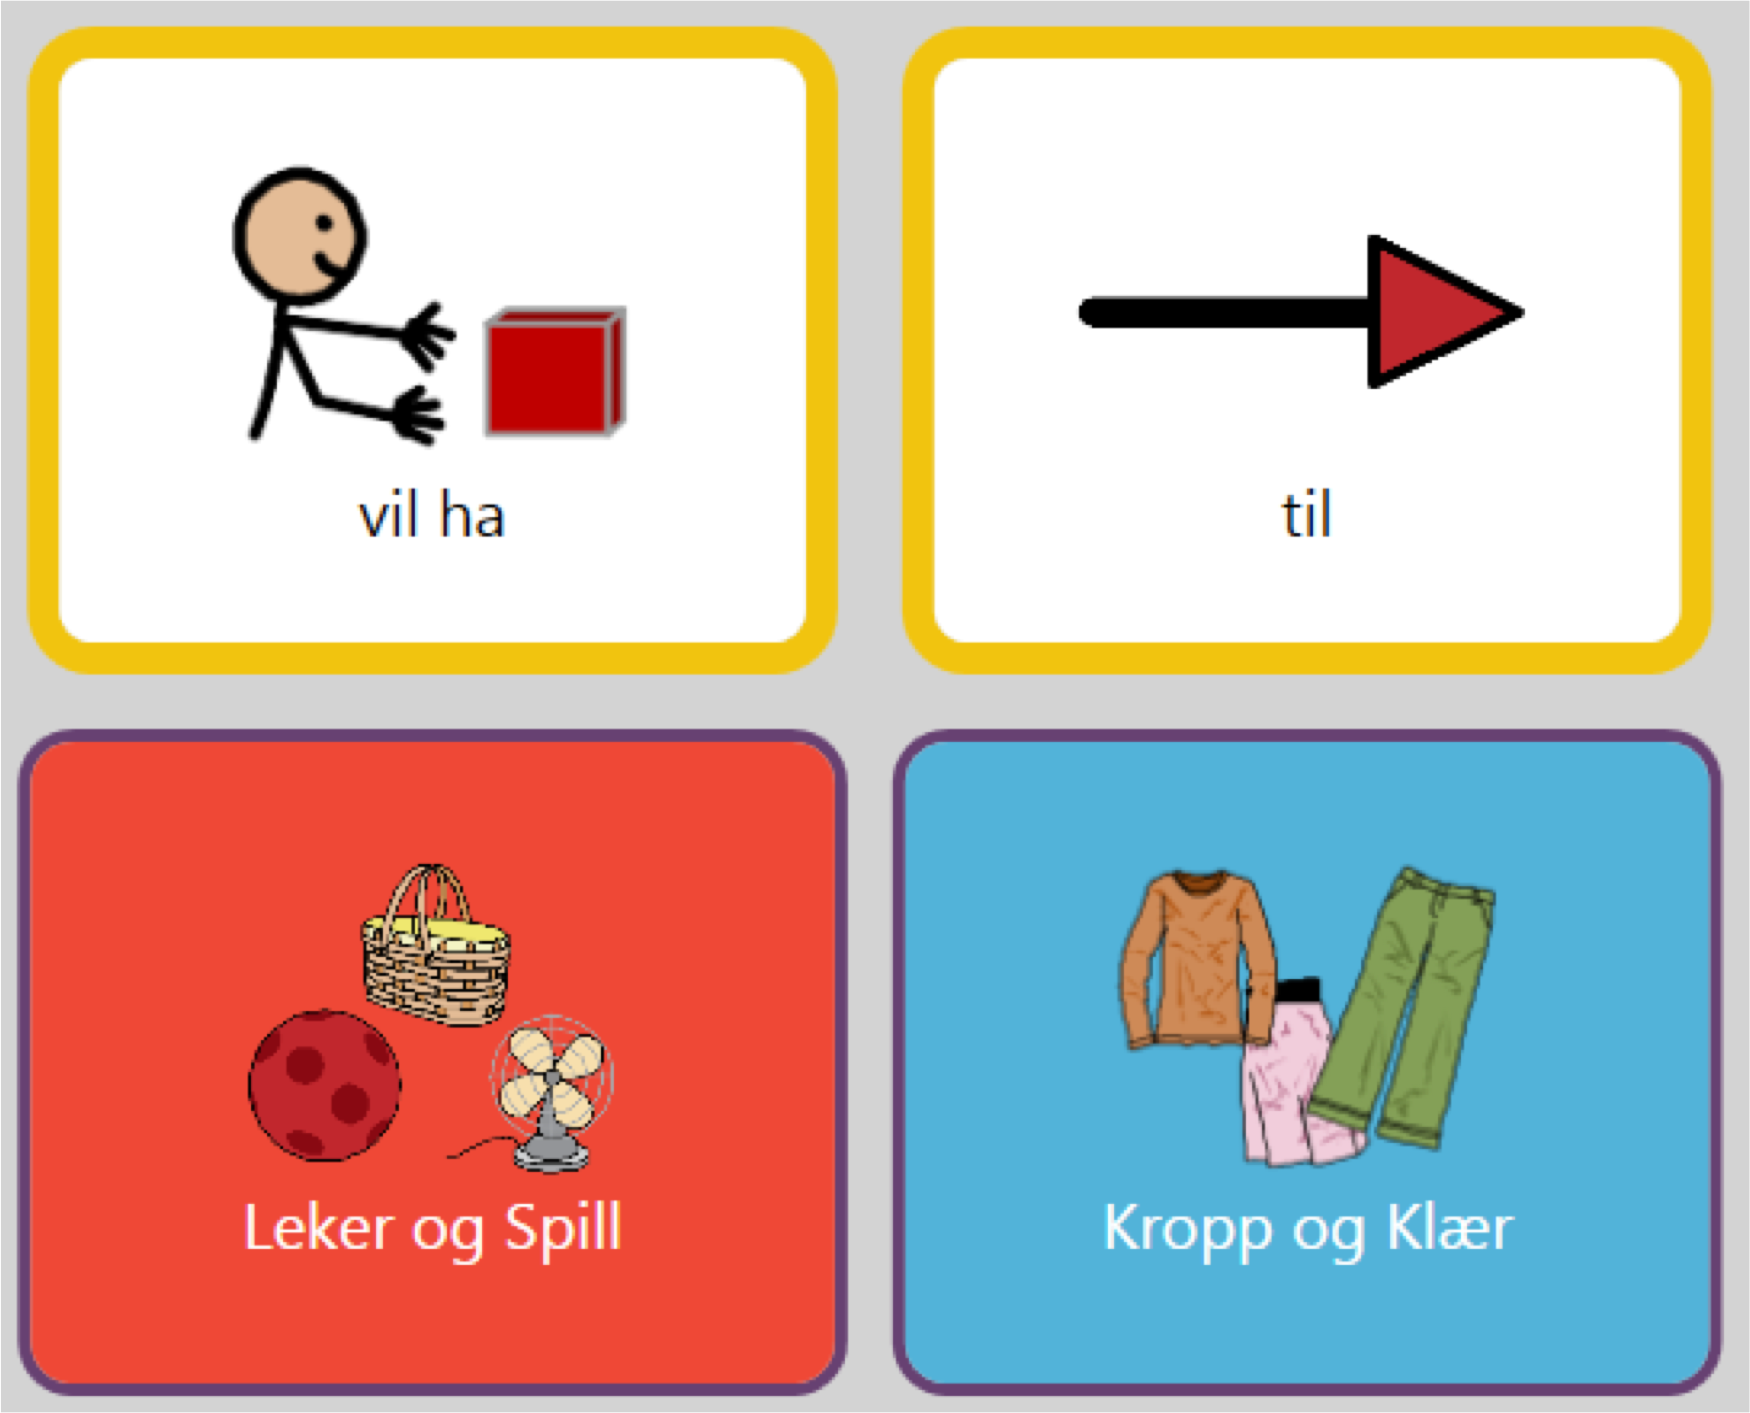
\includegraphics[width=100mm]{Symboler} 
\caption{Fire Symboler vist i brukergrensesnittet} 
\label{fig:symb} 
\end{figure} 

\subsection{SymbolStix}

Bildene som brukes er de samme som i Sono Flex og kommer fra en bildepakke som heter SymbolStix. Dette er en bildepakke som leveres av et eksternt selskap som heter n2y og består av rundt 16 000 symboler \cite{n2y}. Grunnen til at disse bildene ble brukt er fordi det ville tatt for lang tid å lage bilder selv eller å finne dem på nettet, som heller ikke er helt lovlig. Disse bildene har fordelen av at de er laget av profesjonelle noe som ses gjennom den gjennomførte stilen og presise tegninger.


\section{Kategori}

Hver kategori har et navn og en liste over alle symbolene som tilhører den. Eksempelvis så vil symbolene med ord som "hest", "ku" og "hund" ligge i listen til kategorien med navnet "dyr". Figur \ref{fig:katego} viser resultatet ved å trykke på kategorien "dyr". 

\begin{figure}[ht!] 
\centering 
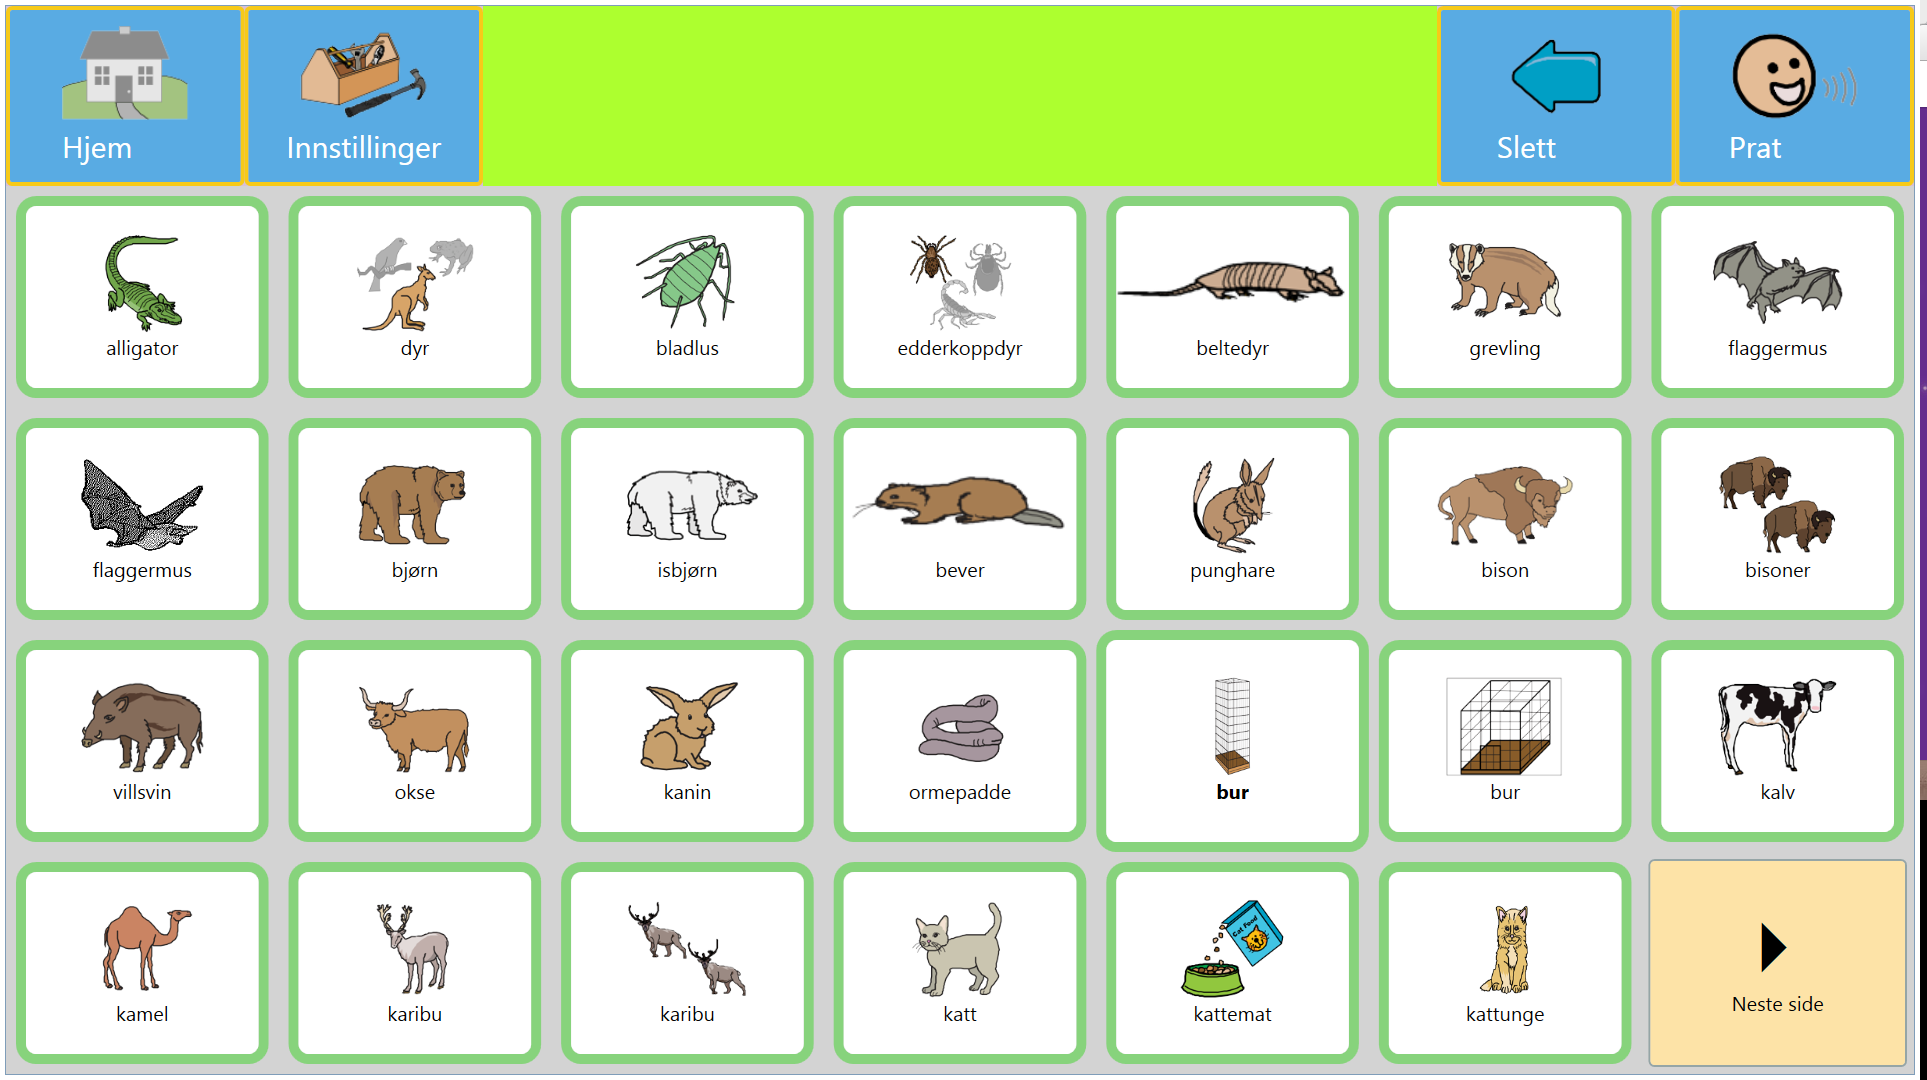
\includegraphics[width=100mm]{dyr} 
\caption{Symbolene på skrivebordet} 
\label{fig:katego} 
\end{figure} 



 
\section{Beskrivelse av prototypen} 

Prototypen har som en kan se fra figur \ref{fig:protooo} den samme layouten som Tobii Sono Flex, med en menylinje etterfulgt av en symboltabell under. Det er derimot en del variasjoner i hver av disse komponentene.  

\begin{figure}[ht!] 
\centering 
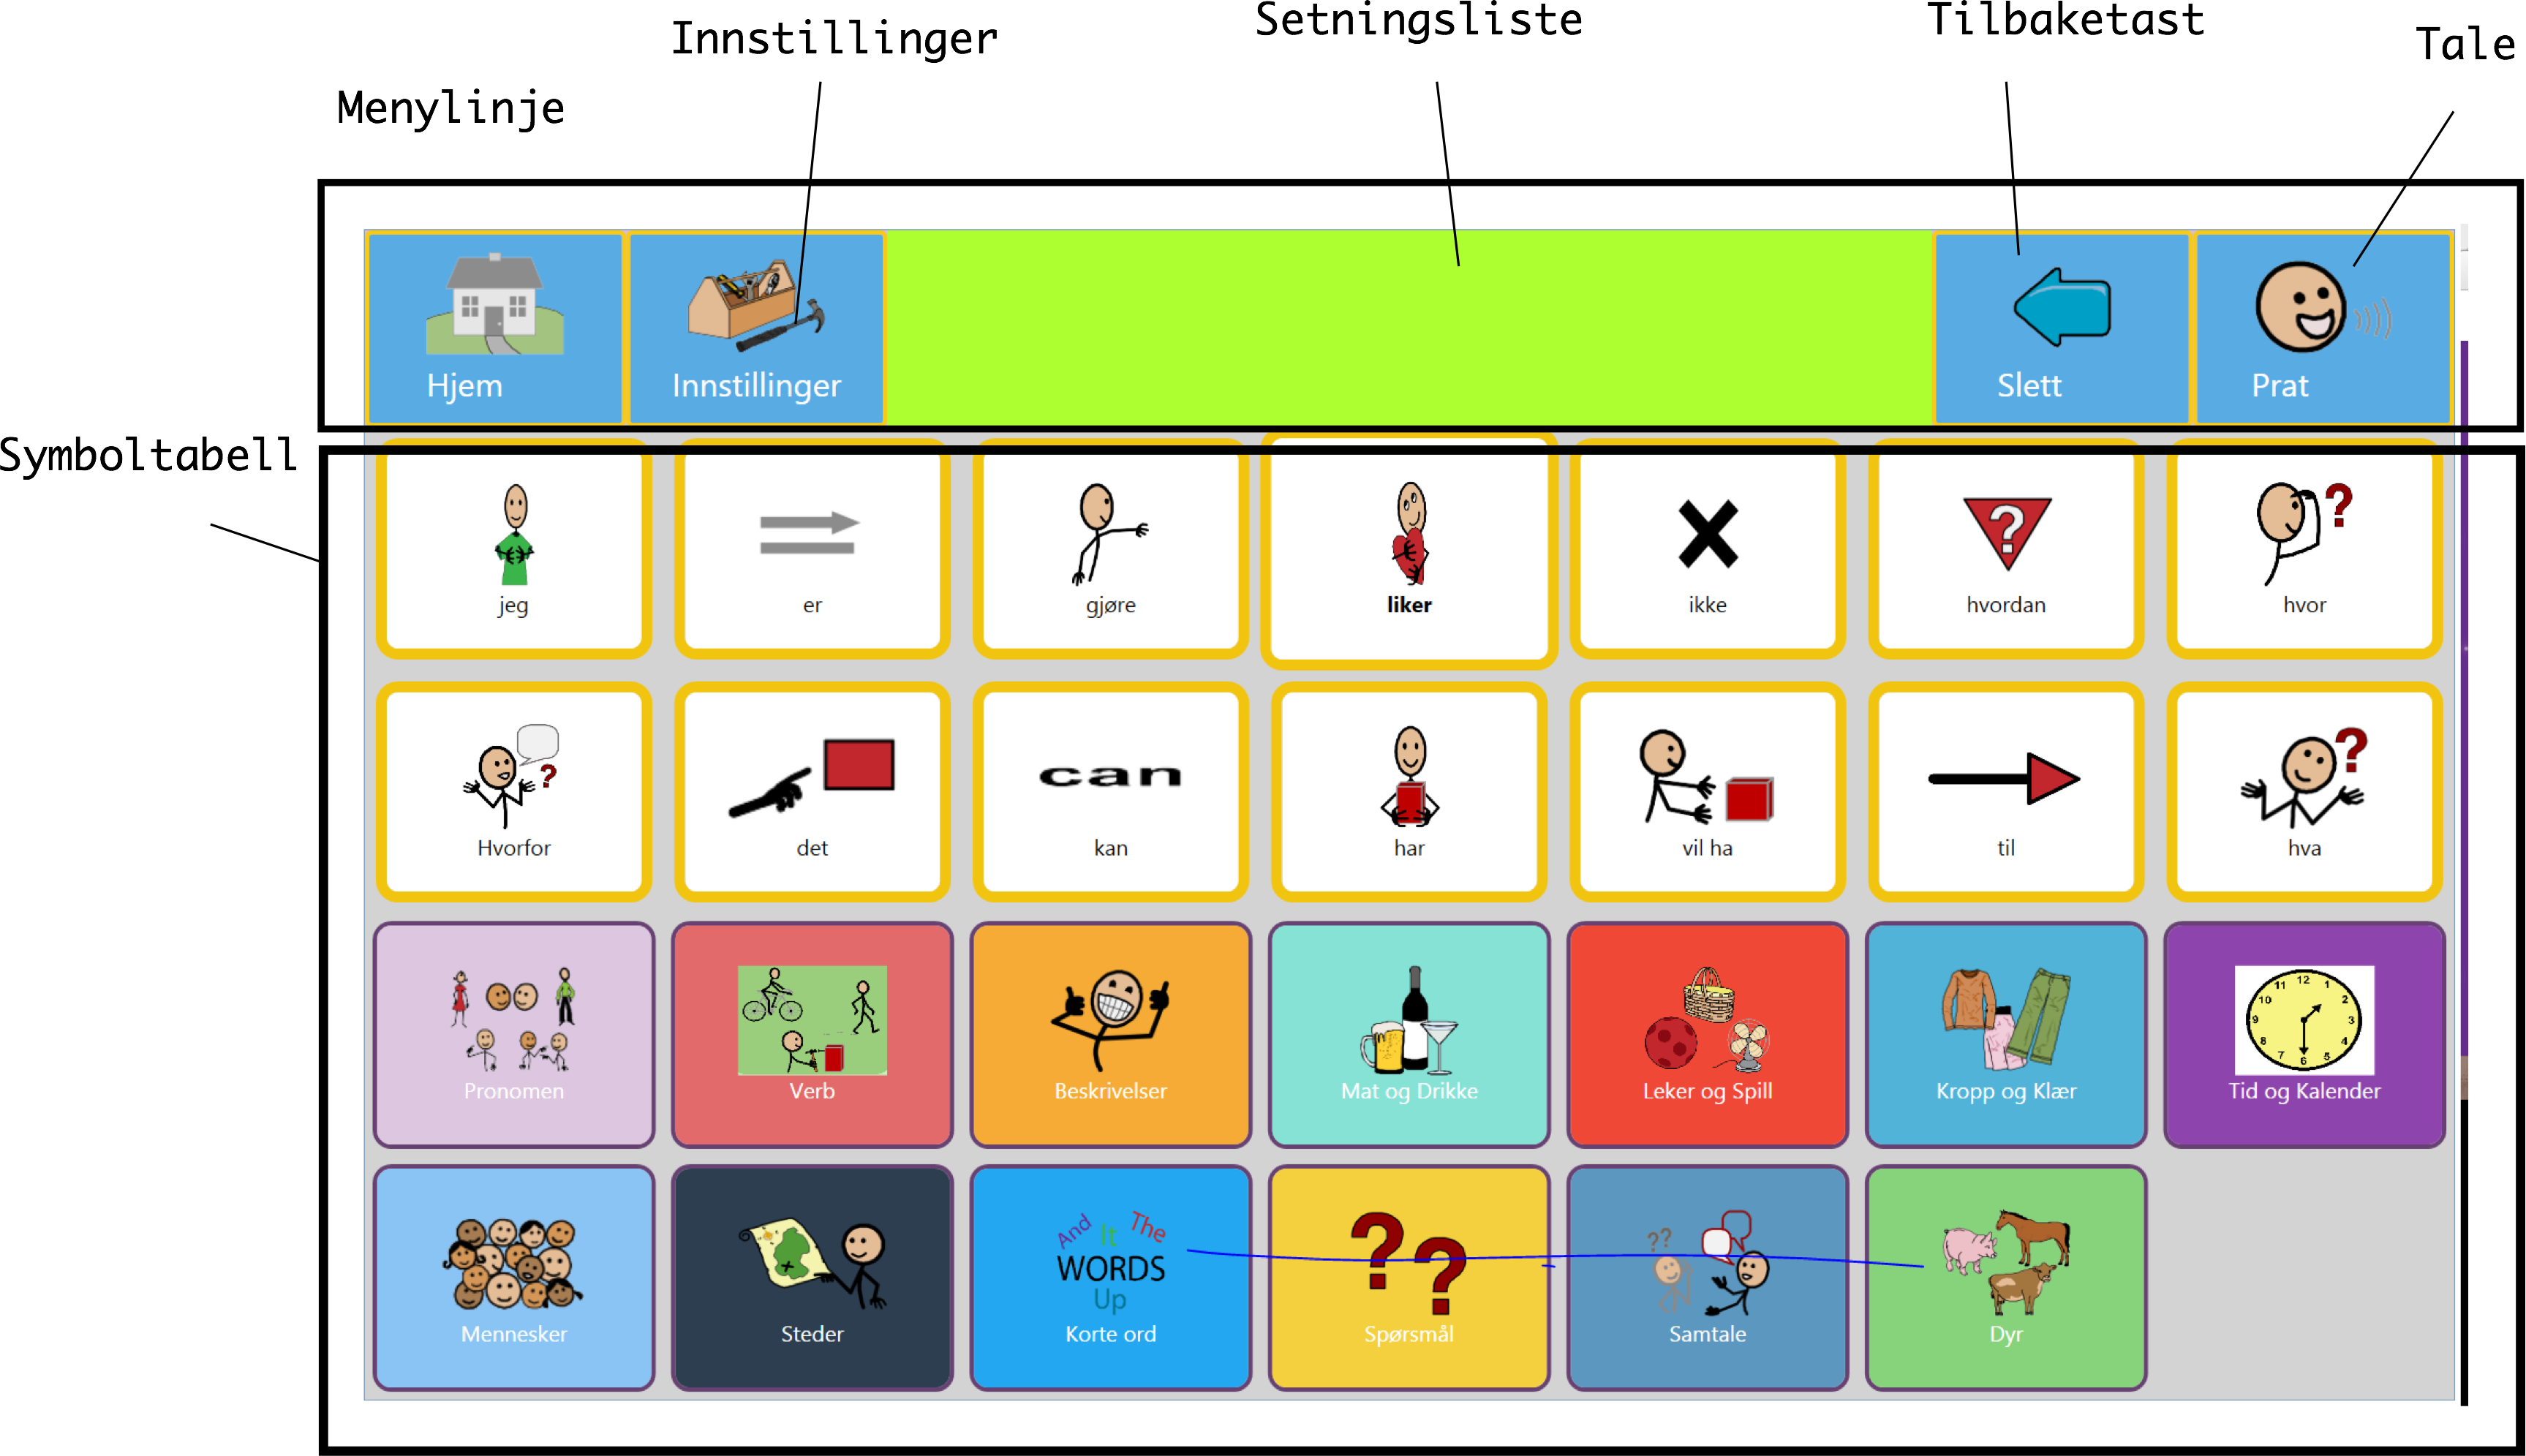
\includegraphics[width=100mm]{ForskjelligeElementerIproto} 
\caption{Prototypen med navn på de ulike delene} 
\label{fig:protooo} 
\end{figure} 


\subsection{Menylinjen} 
 
Menylinjen dekker 1/5 del av applikasjonens vindu og består av 4 knapper og listen over ord som brukeren har trykket på. 
 
\subsubsection{Tilbaketasten} 
 
Tasten som befinner seg til høyre for ordlisten er tilbake tasten. Som på et vanlig tastatur vil et trykk på denne knappen medføre at det siste ordet i ordlisten fjernes. 
 
\subsubsection{Ordlisten} 
 
Når en bruker trykker på et ordsymbol så vil dette legge seg i ordlisten og når han trykker på "prate" knappen så vil ordene i listen bli gitt gjennom høyttalerne som naturlig tale og deretter fjernes fra listen. Selv om det er plass til uendelig med ord i listen så vil det kun være mulig for brukeren å se maks 4 om gangen. Hvis det allerede er fire symboler i listen når brukeren trykker på et nytt symbol, så vil de tre første bli "fjernet" mens det fjerde og det nye symbolet vil være igjen. Hvis brukeren igjen fjerner de to siste ordene ved å trykke på tilbake tasten,  vil ordene som kommer før igjen bli presentert for brukeren i setningslisten.  
 
 
\subsubsection{Hjem} 
Ved å trykke på "hjem" knappen vil brukeren alltid bli ført til førstesiden av applikasjonen uavhengig av hvor han befinner seg.  
 
\subsubsection{Innstillinger} 
Hvis brukeren første er på "hjem" siden av applikasjonen så vil knappen byttes ut med en "innstillinger" knapp. Ved å trykke på denne vil det åpnes et nytt vindu hvor brukeren vil ha mulighet til å sette og endre på diverse innstillinger. Detaljene rundt denne siden er beskrevet i seksjon. 
 
 
\begin{figure}[ht!] 
\centering 
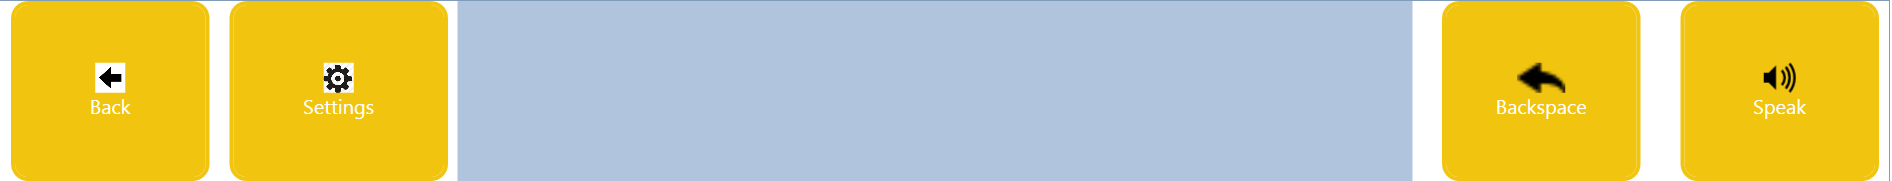
\includegraphics[width=100mm]{MenylinjeP} 
\caption{Skjermdump av menylinjen i prototypen} 
\label{fig:menylinjen} 
\end{figure} 
 



\section{Sammendrag} 

Vi har utviklet en high-fidelity prototype hvor alle kravene i kravspesifikasjonen er oppfylt, noen med mer suksess enn andre. Prototypen er bygget på en moderne plattform som forstatt blir videreutviklet og som har et stort antall tilhengere. Koden skal ved hjelp av flere tiltak være godt tilrettelagt for videreutvikling. 





\chapter{Animasjoner, lyd og brukertilpasning}
 
\section{Animasjon} 
 
 
Animasjoner i programvare brukes som et virkemiddel for å tiltrekke seg oppmerksomhet, underholde eller demonstrere noe. Det kan enten være en kort animasjon der en knapp tiltrer til en side når man svever over den med musen eller det kan være av den lengre sorten som en flash-video.  Animasjon er i hovedsak alt som beveger seg i applikasjonen. Selv om dynamikken som animasjoner kan fungere som et positivt virkemiddel viser undersøkelser gjort av Nielsen og Loranger \cite{NielsenBok}  at for mye blinkende og bevegende elementer kan slite ut brukeren og gjør det vanskeligere å fokusere på oppgaven. Med animasjonene som er implementer ønsker vi å undersøke dette. Hvilke animasjoner fungerer som et hjelpemiddel og med det gir verdi til applikasjonen og hvilke som er distraherende for brukeren og gir en uønsket effekt. 
 
 
I denne prototypen skjer animasjonene som en respons på at brukeren trykker på et symbol. Hva som skjer avhenger av hvilken type symbol det er. De ulike typene som finnes i symboltabellen ble forklart i seksjon \ref{subsubsec:symboltabell}, og er ordsymbol, kategorisymbol og navigasjonssymbol. 
 
 
 
 
\subsection{Animasjoner: ordsymbol} 
 
 
Når en bruker trykker på et ordsymbol, vil symbolet legge seg i setningslisten og er da klar for gjøres om til tydelig tale. Når brukeren har fullført setningen i Sono Flex blir brukeren presentert for endringen ved at symbolet vises i setningsfeltet. Med prototypen ønsker vi  å gi en mer visuell representasjon av denne endringen til brukeren. Ved å la brukeren kunne velge mellom to animasjoner som oppstår når han trykker på ønsket ordsymbol. De to animasjonene fungerer som følgende: 
 

I) Brukeren trykker på et ordsymbol. 
   Ordsymbolet krympes til 5 prosent av størrelsen. 
   I setningslisten vil en kopi av det krympede ordsymbolet dukke opp. 
   Kopien forstørres så til den opprinnelige størrelsen. 
   Ordsymbolet som opprinnelige ble trykket blir forstørret til opprinnelig størrelse. 
 

II) Brukeren trykker på et ordsymbol. 
    Ordsymbolet beveger seg ut av sin posisjon og glir mot den posisjonen den vil ha i setningslisten. 
    Når den har truffet posisjonen i setninglisten, stopper den opp og blir værende i ro. 
 
 
    Med disse animasjonen vil en først og fremst gi brukeren beskjed om at et valg har blitt gjort, men de ønsker også gjøre bruk av programvaren mer spennende.  I Sono Flex  vil ingen av knappene ha noe visuelt som gjør at brukeren kan skille hva som skjer, utenom at symboltabellen bytter ut de eksisterende symbolene. I dette tilfelle vil en se at symbolet går fra å være en statisk symbol til å bli flyttet til setningslisten og bli en del av ønsket setning.  
 
 
 
 
 
 
\subsection{Animasjon: Kategorisymbol} 
 
 
Når en bruker trykker på et kategorisymbol vil symbolene i symboltabellen byttes ut med symbolene som hører til i den gjeldene kategorien. Hvis en trykker på kategorien "dyr" så vil tabellen fylles med ordsymbol som "Hund", "katt", "tiger" o.s.v. Her ønsker animasjonen å hjelpe til med å fortelle at man ikke trykker på ordet dyr, men kategorien dyr og at brukeren får en forståelse for forskjellen mellom dem. Animasjonen startet ved at symbolet som brukeren trykket på forstørres helt til den dekker hele symboltabellen. Det vil si at ingen av de andre symbolene vises, kun kategorisymbolet. Symbolet vil så igjen forminskes, men symbolene i tabellen vil være erstattet av symbolene som tilhører kategorien.  
 
 
 
 
\subsection{Animasjon: Navigasjonssymbol} 
 
 
Den siste typen symbol er navigasjon og ved interaksjon vil den navigere mellom sider når det ikke er plass til alle symbolene på en side. Det vil si at symbolet skal kunne navigere fremover, fra side 1 til 2 og 2 til 3 og bakover igjen. Når brukeren trykker fremover starter animasjonen ved at alle symbolene som er på gjeldene side og neste side begynner å bevege seg mot venstre. Slik at symbolene på gjeldene side kontinuerlig blir byttet ut med de på neste. Symbolene på siden sklir ut, mens symbolene på neste sklir inn og overtar plassene. Når brukeren nå trykker på bakover-symbolet vil det samme skje bare at symbolene sklir mot høyre. 
 
 
\section{Lydeffekter} 
 
 
Som en del av rapporten ønsket vi å undersøke hvilken påvirkning lydeffekter hadde på brukeren. Hovedsakelig var målet å finne ut to ting. I hvilken grad hjelper effektene brukeren i å navigere rundt i applikasjonen og om det vil påvirke brukerens helhets uttrykk av applikasjonen.  
 
 
\subsection{Lydeffekter i prototypen} 
 
 
I prototypen er det lagt til flere lydeffekter, utelukkende i form av små lydklipp på maks 1 sekund. Effektene vil kun bli avspilt som en respons til noe brukeren foretar seg eller som å informere om en hendelse. Denne begrensning finnes for å ikke skape forvirring hos brukeren. Hvis lyd også hadde blitt avspilt tilfeldig så ville meningen med effektene forsvinne. Fordi brukeren blir lurt til å tro at programvaren har registrert en interaksjon, selv om han ikke har foretatt seg noe. Det er derfor viktig at det er lett for brukeren å skille mellom effektene som representerer en interaksjon og informasjon. De ulike interaksjonslydeffektene er også forskjellige, og hvilken som blir spilt er avhengig av,  som med animasjon,  hvilken type komponent brukeren samhandler med. Eksempelvis vil lyden som blir avspilt når brukeren trykker å tilbaketasten representere noe som forsvinner.  
 
 
 
 
\begin{itemize} 
\item Symbolord - Enkel klikkelyd 
\item Kategoriord - usikker 
\item navigasjonsord - svisj 
\item Innstillinger - Verktøyskasse 
\item tilbaketasten/slett - forvsinner 
\item hjem - usikker 
\item prat 
\end{itemize} 
 
 
 
Dette vil forhåpentligvis gjøre at brukeren mer effektivt kan bekrefte valget og fortsette med oppgaven. Som  
 
Hvilken brukeren blir presentert for er avhengig av hvilket komponent han interagerer med.  Grunnen er at hvis effektene hadde blit avspilt uten at brukeren foretar seg noe, så kan 
 
Hvilken lyd som blir avspilt er avhengig av hvilket valg brukeren har foretatt seg, og responsen til brukeren vil  
 
Eksempelvis hvis brukeren foretar seg et ulovlig valg vil han bli presentert for en lyd som har gir negative assosiasjoner.  D 
 
Lyden som vil bli gitt til brukeren vil komme i form av små lydklipp som maks vil vare i et sekund,  ettersom det skal være nok for at brukeren kan registrere det.  
 
 Tilbakemelding i form av lyd gir brukeren en bekreftelse på at han valget han nettopp har foretatt har blitt registrert og  
 
Ta for eksempel brødristeren. Når den er ferdig vil brødet hoppe opp, men i tilegg vil den gi fra seg et pling. Altså brukeren vil få tilbakemelding på at han kan hente brødet både visuelt(brødet som hopper opp) og gjennom lyd(plinget). Ved å g 
 
Lyd brukes ofte for å fortelle brukeren av produktet noe. For eksempel vil brødristen gi fra seg et pling når den er ferdig samtidig med at skivene hopper opp av maskinen. I dette tilfellet vil  
 
 
I dag brukes lyd ofte i flere sammenhenger, i alt fra 
 
 
 

 
 
\chapter{Testing} 
 
\section{Introduksjon} 
 
En viktig del av rapporten var å teste ut hvordan animasjoner og lyd påvirker barns opplevelse av programvaren når de bruker en øyesporingsenhet til interaksjon med maskinen. En fremgangsmåte vil vært å teste på et utvalg studenter og tolke disse resultatene. 

Problemet er at resultatene ikke nødvendigvis vil være det samme for barn som med voksne. Som tidligere referert, mens barn finner animasjon og lyd interessant og spennende, vil voksne være mindre positive og kan til og med finne dem irriterende. Det ble derfor bestemt at deltakerne i  hvertfall måtte være i nærheten av alderen til målgruppen for at det skulle være noe poeng med testingen. 

Testen ønsket spesielt å utforske to ting. Den første var å finne ut om målgruppen greide å bruke prototypen. Ville de greie å navigere og utføre de mest nødvendige oppgavene som å skrive en setning, fjerne ord og gjøre det om til tale. Den andre var som tidligere nevnt, å finne ut effekten animasjoner og lyd har når barn skal bruke programvaren.  
 

\section{Rekruttering av testere} 
 
 
For å rekruttere deltakere til testen ble først pedagogisk avdeling ved Høgskolen i Bergen kontaktet. De hadde tidligere hatt erfaring med å teste på den ønskede målgruppen. Målet var at disse kunne sette oss i kontakt med nøkkelpersoner og i tillegg gi retningslinjer og tips angående det å bruke barn med funksjonshemninger til undersøkelser. 

Gjennom dette møte ble vi satt i kontakt med Pedagogisk-psykologisk Tjeneste (PPT). PPT er kommunal tjeneste som skal hjelpe barn, ungdom og voksne som strever i utviklingen, eller som har en vanskelig opplæringssituasjon. De skal hjelpe ved å gi systemrettet støtte, med råd og veiledning til skoler om pedagogisk ledelse av gruppe- og læringsmiljø, og bistand med kompetanse- og organisasjonsutvikling \cite{Udir.5:online}. De hadde god erfaring med målgruppen og hadde et større kontaktnettverk enn høgskolen. 

Gjennom PPT ble det sendt ut et informasjonsskriv (se vedlegg A) til foresatte av barn som passet inn i målgruppen hvor det ble gjort rede for hvordan undersøkelsen ville bli gjennomført og hvilke og hvor lenge data ville bli lagret. For at testingen skulle gjennomføres, måtte en av barnets foresatte signere og returnere skjemaet. Dessverre var det ingen av de foresatte som ønsket at barnet skulle delta i undersøkelsen. Vi ble derfor enige om at programvaren uansett måtte testes og at det nærmeste da ville være barn i samme alder som målgruppen, men uten funksjonshemningene.  Det ble etter en kontaktrunde klart at seks foresatte med barn ved Krohnengen barneskole hadde gitt sin tillatelse til å la barna delta i undersøkelsen. 
 
 
\section{Gjennomføring av test} 
 
 
\subsection{Pilottest} 
 
Før testingen ble det utført en pilottest på skolen med 4 medstudenter. Dette ble gjort for at testingen skulle gå best mulig og for å identifisere tekniske feil og eventuelle andre hindringer som kunne oppstå underveis.  
 
 
\subsection{Sted} 
Testen ble utført på Krohengen barneskole inne på biblioteket mellom klokken 13:00 - 
16:00. Bilde \ref{fig:test_lokale} viser et bilde av testrommet. Dette rommet ble valgt fordi det var nært barnas oppholdsrom og fordi det var 
stille. Det var ingen andre barn utenom deltakeren i rommet da testen ble utført. 

 
 
\begin{figure}[ht!] 
\centering 
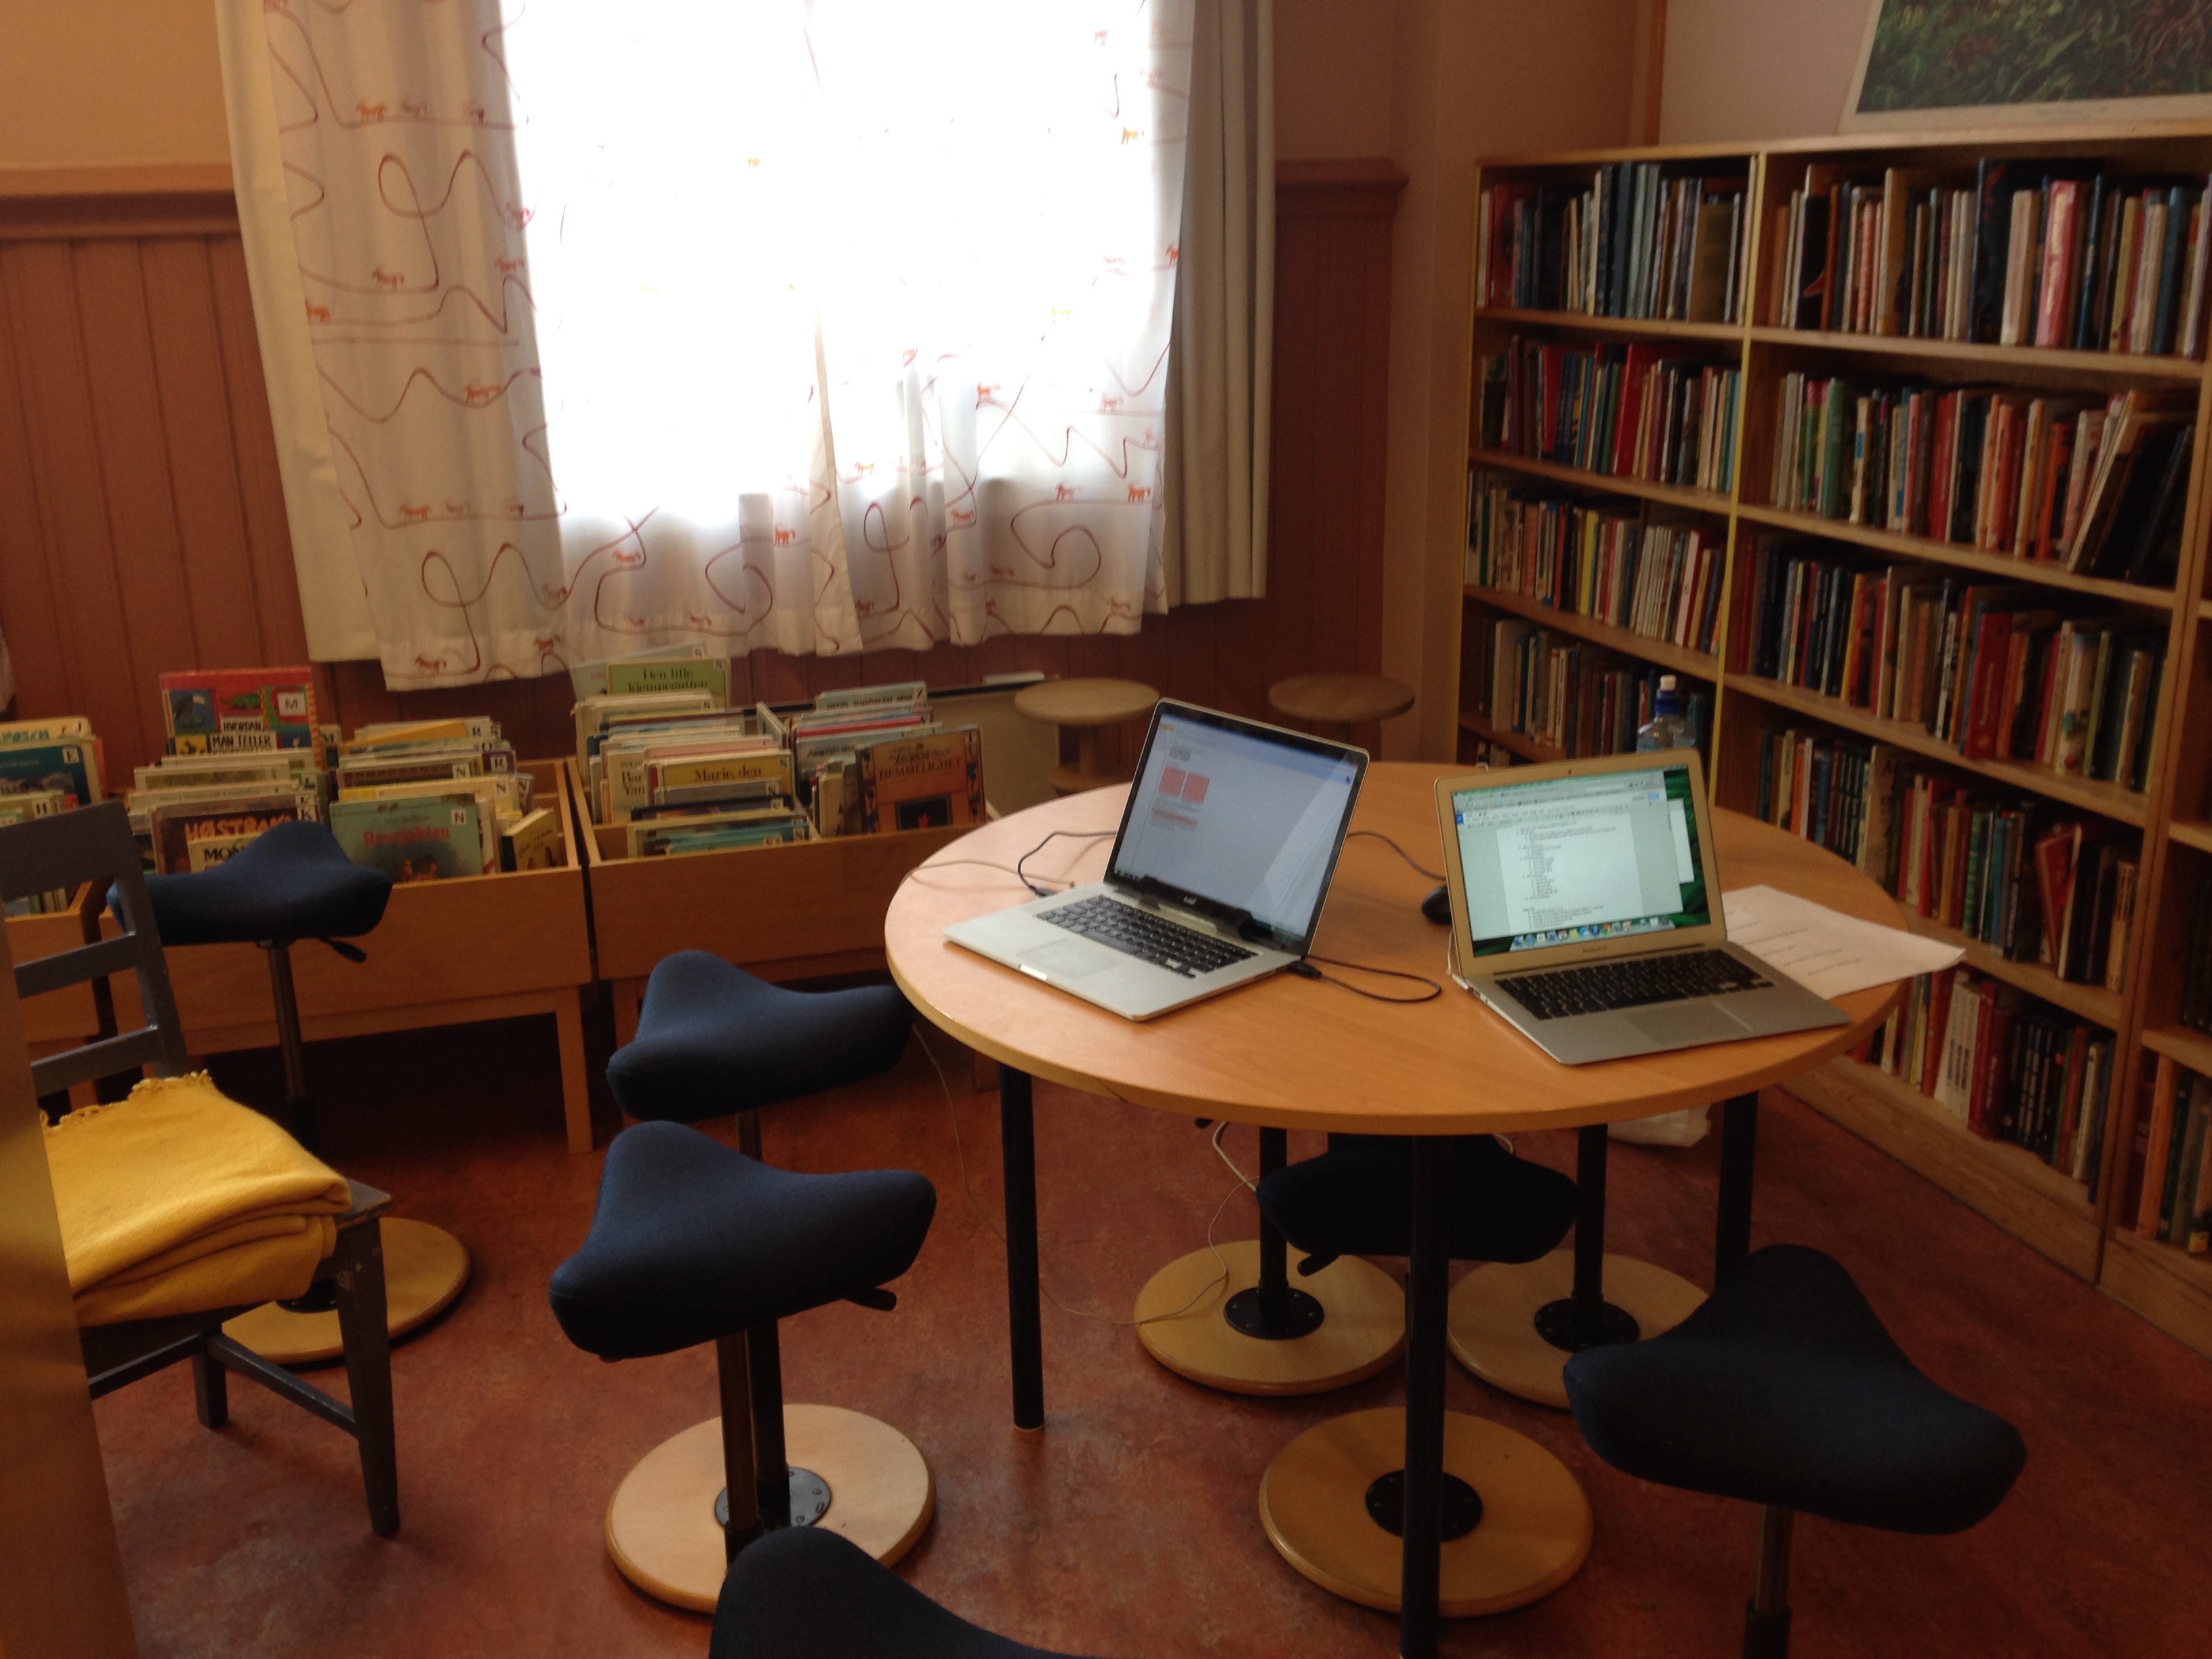
\includegraphics[width=100mm]{Lokale} 
\caption{Bilde av testlokale} 
\label{fig:test_lokale} 
\end{figure} 
 
 

\subsection{Testgjennomføring} 
Hver test ble gjennomført ved at et og et barn kom inn i biblioteket hvor det først ble foretatt en kort 
samtale for at barnet skulle føle seg komfortabel. For å unngå distraksjoner var kun deltaker og testleder 
tilstede under testingen. Barnet ble plassert foran datamaskinen og øyesporingsenheten satt slik at den siktet på deltakerens ansikt. For at øyesporingsenheten skulle bli mest nøyaktig måtte den tilpasses for hver deltaker ved en kalibreringsprosess. Prosessen foregikk ved at brukeren følger en rød prikk som starter i 
venstre hjørne og traverserer over skjermen to ganger før den stopper nede i høyre hjørne. Dette 
tar cirka 30 sekund. Etter hver test ble det gitt en farge som beskrev hvor godt enheten greide å 
tilpasse seg brukeren. Rødt er dårligst og programvaren vil ha vanskeligheter med å regne ut hvor 
brukeren ser på skjermen. Gul vil si at kalibreringen gikk greit og at brukeren skal kunne bruke 
enheten på en god måte. Grønn er den mest nøyaktige kalibreringsgraden og enheten vil presist 
fange opp hvor brukeren skuer. Hvis en bruker fikk kalibreringsgrad rød, ble prosessen gjentatt en 
gang. Hvis det igjen viste seg å bli rød ble brukeren bedt om å bruke mus. Kalibreringsgraden ble 
notert for alle brukerne. Deretter ble programvaren startet, og brukeren fikk lov å prøve programvaren før selve testen startet. 
 
 
Testen startet med at brukeren ble  gitt 5 oppgaver som skulle gjennomføres. En bruker ble kun presentert for en ny oppgave når den forrige var fullført. Hver oppgave hadde en makstid på 5 minutter. Det vil si at hvis deltakeren brukte mer enn dette, ville oppgaven bli registrert som feil og avsluttet. Brukeren ville så bli tildelt neste oppgave. Denne makstiden ble valgt utfra pilottestingen. Der brukte deltakerne ca. 30 sekund per oppgave, og med tanke på at disse var i 20 årene ble det også lagt til en god sikkerhetsmargin. Under testingen ble det forsøkt å gi minst mulig spørsmål og ledetråder for å ikke forstyrre eller hjelpe brukeren ettersom dette ville ha påvirket resultatet. Når brukeren hadde gjennomført alle oppgavene ble han stilt 5 spørsmål. Til slutt ble deltakeren takket for deltakelsen og tildelt et trekk til sykkelsete som takk for hjelpen. 
 
 
\section{Datainnsamling} 
 
 
For å samle inn data ble det brukt flere ulike metoder.  
 
 
\subsection{Loggfører} 

En viktig del av undersøkelsen var å se hvor lang tid og hvor mange trykk deltakeren brukte på å utføre de forskjellige oppgavene som han ble tildelt. For å gjennomføre dette ble det brukt en logger som lagret data for hver test på separate tekstfiler. Grunnen til at en logger ble brukt er fordi data lagres i et standardformat som gjør at en enkelt kan kjøre spørringer og dermed hente ut målbar data. Data lagres også med en presisjon på tid som en menneskelig observatør ikke har mulighet til og er ikke like mottakelig for feil. Den har også den fordelen at den ligger i bakgrunnen uten at brukeren merker noe til den, samtidig som den ikke har noen merkbar innflytelse på programvarens ytelse. 
 
 
For hver test ble det ved starttidspunktet logget om animasjoner er på eller av, alderen til barnet og om den nødvendige kalibreringen er fullført. Deretter var det kun data fra interaksjoner brukeren gjorde med programvaren som ble lagret. Ettersom brukeren kun har mulighet til å trykke på brikker kan det forenkles til at hver gang deltakeren trykket på en brikke ble data logget. For hvert trykk på en brikke ble det lagret hva som sto på brikken, hvilken type brikken var av og tidspunktet. 
 
 
\subsection{Skjermopptak} 
 
Loggeren fanger kun opp interaksjoner deltakeren gjør med programvaren, noe som utelater det som skjer imellom hver interaksjon. For å kompensere for dette ble det bestemt å ta i bruk en skjermopptaker som kunne fange opp hendelser mellom trykk. Noe som kunne være interessant for å se hvor brukeren "nesten" trykket og hvordan han beveget blikket, og generelt andre unntak som måtte oppstå. En stor ulempe med skjermopptak er at en observatør fysisk må se igjennom opptaket for å kunne hente ut informasjon. Noe som kan bli ressurskrevende.
 
Skjermopptakeren ble som med loggeren startet på nytt for hver test og lagret som separate mp4 filer.  
 
 
\subsection{Observasjon} 
 
For å senke terskelen for at foresatte skulle tillate barna å delta i testen ble det valgt å ikke filme barna under testing. Dette gjorde derimot at en ikke fikk med seg reaksjoner eller spørsmål som ble stilt underveis. For å kunne fange opp dette ble det brukt en observatør til å notere ned eventuelle hendelser og spørsmål som deltakeren måtte gjøre seg underveis. Ulempen med dette er at man ikke har samme mulighet som med film til å undersøke det i ettertid. Hvis man går glipp av noe er det ikke mulig å spole tilbake for å se det igjen. Det kan også virke forstyrrende på en deltaker at en person noterer det han foretar seg. 

 
\subsection{Intervju} 

Etter at deltakeren har gjennomført oppgavene vil det bli gjort et kort semi-strukturert intervju. Det vil si at spørsmålene er forhåndsdefinerte som i en undersøkelse, men med mulighet for å komme med oppfølgingsspørsmål for å få klarhet i svarene. Intervjuet ble gjort for å undersøke ting som det ikke var mulighet til å fange opp med automatiske verktøy. Blant annet hvordan brukeren opplevde programvaren og hva han syntes om den. 
 
\section{Oppgaver} 

Som en del av testen ble deltakerne gitt oppgaver som går ut på enten å finne frem enkle ord eller kombinere flere ord til å bygge setninger. For at å kunne gi det beste sammenligningsgrunnlaget ble alle deltakerne tildelt de samme oppgavene. 
 
Den første oppgaven var å finne ordet "hvordan". Denne brikken ligger på første siden og skal være enkel å finne. Meningen med dette er at deltakeren skal forstå hvordan oppgavene er oppbygd og samtidig få litt selvtillit til de neste oppgavene. 
 
Den andre oppgaven var litt verre, den gikk ut på at man skal finne brikken hvor det står "banan". For å finne denne må man først trykke inn på kategorien "Mat og Drikke" for å finne brikken med "banan", som i dette tilfelle vil være på den første siden inne på kategorien. Vanskelighetsgraden vil øke en del fra første oppgaven, men antagelsen var at det skal være enkelt å forstå at en må trykke på kategoriknappen "mat og drikke" for å finne ordet "banan". I hvertfall i motsetning til mer abstrakte kategorier som "verb" og "pronomen". 
 
Tredje oppgaven var å finne brikken hvor det står "Elg". På samme måte som med "banan" må man også her først finne den passende kategorien. Antagelsen var også her at det skal være en ganske grei oppgave å finne for barna, med tanke på at den ligger under kategorien "dyr". Forskjellen her i forhold til forrige oppgave er at man ikke vil finne brikken på første siden etter at man har trykket på kategorien "dry", man må navigere seg over til neste side. Dette er om barna forstår konseptet med sidenavigering.
 
I den fjerde oppgaven ønsket vi at deltakeren skulle skrive "Jeg vil ha banan", og er med det den første oppgaven hvor deltakeren måtte kombinere ord for å bygge en setning. Det ble derfor valgt en rimelig enkel setning der de to første brikkene "jeg" og "vil ha" er lokalisert på den første siden, det siste ordet har deltakeren funnet en gang før. Dette er gjort for at vanskelighetsgraden ikke skal øke for fort når brukeren skal gå fra å finne et ord til flere.
 
Den femte oppgaven gikk ut på at deltakeren skulle skrive setningen "Jeg liker katt". Igjen vil de to første ordene være på den første siden. Mens det andre ordet "katt" vil finnes under kategorien "Dyr". En kategori barnet tidligere var innom i tredje oppgaven når han skulle finne "Elg". 
 
 
\section{Resultat} 
 
\subsection{Observasjon} 
 
Hver test startet ved at SFO-lederen hentet neste deltaker fra oppholdsrommet og tok dem med til biblioteket hvor undersøkelsen fant sted. De ble der presentert for testlederen av en SFO ansvarlig for at barnet skulle føle seg trygg. Det ble stilt et par enkle spørsmål, hovedsakelig for å lette på stemningen. Det ble også undersøkt om noen av barna hadde prøvd øyesporing før, noe som hadde gitt dem en stor fordel. Det var derimot ingen av dem som hadde erfaring med øyesporing. 
 
 
Før selve testen startet, ble testdeltaker satt på en stol foran datamaskinen med programvaren og bedt av testleder om å kalibrere øyesporingsenheten. Kalibreringen gikk som tidligere nevnt utpå å følge en prikk som gikk frem og tilbake over skjermen. Her valgte flere av deltakerne å bevege hodet mer enn øyene, og ble dermed bedt om å prøve å holde hodet stille. Flere reagerte på dette med å stirre intenst på prikken som fløyt over skjermen, noe som gjorde at deltakerne i etterkant fikk litt vondt i hodet. I tre av tilfellene gikk kalibreringen såpass dårlig at den måtte gjentas. Dette virket negativ inn på barna og de laget lyder med negative assosiasjoner. I et tilfelle ble også den andre runden med kalibrering for dårlig, slik at det ikke ville gitt meningen å bruke øyesporing. Det ble derfor bestemt at deltakeren skulle gjennomføre testen med data mus. Dette ble notert og vil bli tatt hensyn til i evalueringen av data. 
 
Når kalibrering var ferdig, ble programmet startet. Her ble deltakeren først presentert for en introduksjonsskjerm og bedt om å velge sin alder av et utvalg på 3 knapper. Her var det flere som med en gang rakk mot styringsflaten for å trykke på knappen med fingrene, ettersom de ikke var vant til å styre med øyene. Det var derimot det eneste tilfelle hvor testleder måtte gjør deltakerne oppmerksom på at de skulle bruke øyene. 
 
Når brukeren var ferdig med introduksjonen starter det som er selve programvaren og som skal testes. Her ble hver deltaker oppfordret til og prøve å trykke på et par knapper med øyene for å bli kjent med følelsen og hvordan interaksjonen fungerte. Den første oppgaven ble gitt til deltakerne, finn brikken hvor det står "Hvordan". Det kunne da virke som om flere av deltakerne ble litt stresset. For mens de lette rundt på skjermen etter den korrekte brikken begynte tiden på hver brikke å gå. Det vil si hjulet som sier hvor lang tid som gjenstår før det blir registrert som et klikk. Dette gjorde at de ble tvunget til raskt å flytte blikket rundt for å unngå trykk på uønskede brikker. Det kunne se ut som om tidtakeren som begynner når en bruker ser på en brikke tok veldig mye oppmerksomhet vekk fra den faktiske oppgaven, som var å lete etter rett brikke. Dette gikk igjen under alle oppgavene og gjaldt for alle deltakerne. Dette er nødvendigvis ikke noe som kun gjelder på barn ettersom vi også ble oppmerksom på denne tendensen under pilottesten på eldre deltakere. Opptil flere ganger gikk tidtakeren helt ut på feil brikker, som gjorde at programvaren registrerte det som et trykk og brikken ble flyttet til setningslisten. En deltaker  der animasjoner var slått på, brukte brukeren tid på fjerne feil trykk ved å trykke på tilbaketasten, mens de andre lot feiltrykk være. Testleder ga aldri noen hint om at deltakerne trengte å gjøre dette.  
 
 
Andre oppgaven var å finne ordet "banan", noe som økte vanskelighetsgraden et hakk ved at barnet først måtte finne den passende kategorien, før han kunne finne rett brikke. Som med den første oppgaven begynte de å lete etter brikken i leseretning. Testleder spurte deltakerne under denne oppgaven om å se på bilde eller lese teksten under for å finne rett brikke. Ingen av deltakerne ble forklart at flere av brikkene var kategorier, noe som gjorde at de etter å ha sett over alle brikkene kunne opplyse at de ikke kunne finne brikken hvor det sto "banan". Det ble da gitt et tips fra testleder om at noen brikker kunne gjøre slik at det dukket opp flere og at de måtte finne den. Når det var sagt, var det ingen som brukte lang tid på finne fram til den korrekte kategorien og deretter finne banan brikken.  
 
 
Etter å ha skrevet banan ble de bedt om å finne brikken hvor det sto elg. Deltakerne så da ut til automatisk å lete blant kategori brikkene og tiden som ble brukt på å finne rett kategori var kort. Problemet var at brikken hvor det sto elg ikke befant seg på den første siden, men andre. For å komme til denne må en navigere seg til neste side. Her varierte det svært mellom deltakerne. En skuet over alle brikkene og når han ikke fant den ønskede, navigerte han seg tilbake til forsiden istedenfor til neste side. En annen deltaker hadde derimot mer korrekt fremgangsmåte. For etter raskt å ha konstatert at brikken ikke fantes på den aktuelle siden, trykket han til neste side og fant brikken.  
 
Med de tre første oppgavene unnagjort skulle deltakerne kombinere det de hadde lært ved å skrive den enkle setningen "jeg vil ha banan". Ingen av barna hadde noe særlig problem med å finne de to første ordene, og det tredje hadde alle allerede funnet en gang, men allikevel var det to som ikke automatisk kom på dette og igjen begynte å se over kategoriene. Alle så ut til å håndtere overgangen fra enkle ord til setninger svært bra, slik at når de kom på tredje oppgaven som var å skrive "Jeg liker katt" begynte de med en gang uten noen videre beskjeder fra testleder å finne frem til de korrekte knappene. Til tross for at de ikke hatt brukt brikken "katt" før, fant de raskt frem rett kategori. Det som var interessant, var at flere valgte feil brikke til tross for at de var på rett side. Grunnen til dette er at inne på første siden finnes det i tillegg til brikken hvor det står "katt" også en brikke hvor det står "kattunge". Det som skjedde var at samtlige av testdeltakerne valgte sistnevnte. På spørsmål fra testleder om hvorfor de gjorde dette, var det en som svarte at oppgaven var å finne "katt". Deltakerne ble derfor spurt om de baserte brikketrykkene sine på teksten eller bildet. Hvor samtlige av barna svarte bildet. Noe som ikke bare forklarte hvorfor de valgte "kattunge", men også hvorfor det virket lettere for deltakerne å finne kategorien "dyr" enn "mat og drikke". For mens "dyr" var representert med ulike bilder av dyr, var "mat og drikke kun representert av drikkevarer. Noe vi ble oppmerksom på i etterkant. 
 
Til tross for at ingen av deltakerne hadde brukt øyesporing før, fikk alle det til, med unntak av deltakeren der kalibrering ikke fungerte. Ingen feil dukket opp og alle deltakerne greide å gjennomføre oppgavene. Selv om det var relativt få oppgaver greide de dem uten noe særlig behov for å tenke seg om. På bakgrunn av observasjonene kan en slå fast at for en førstegangsbruker kan tidtakeren som vises gå litt for raskt og en bør muligens se på alternative måter å vise denne, fordi det skjedde flere feiltrykk og deltakerne ble stresset og ikke visste hvor de skulle hvile blikket mens de lette etter ønsket ord. Det kan også konkluderes med at de i hovedsak bruker bildet til å finne rett brikke noe som gjør at bildet bør vise klart hva det representerer for unngå tvetydighet.  
 

\subsection{Intervju} 
 
Med det semi-strukturerte intervjuet ønsket vi å finne ut hvordan barna opplevde å bruke prototypen. Problemet var at uansett hvordan spørsmålet ble formulert var deltakerne utelukkende positive. Eksempelvis ga alle karakteren 10 på en skala fra 1 til 10, og på oppfølgende spørsmål om det var ingenting som burde vært annerledes, var svaret nei. Dette gjorde at flere av spørsmålene som ble stilt ble forkastet.  
 
Et spørsmål som var av interesse var når testlederen spurte barna om de visste hva som skjedde ved å trykke på de ulike knappene. Det vil si om de forsto om det var et ord eller kategori. To av dem svarte klart at ved å trykke på en kategori knapp, ville knappene bli byttet ut med nye knapper. Mens ved å trykke på et symbol som representerte et ord, ville det gå opp i setningslisten. De andre greide derimot ikke å svare på dette spørsmål og greide ikke å skille mellom de ulike knappene. 
 

\subsection{Tid} 
 
 
En ting som vi ønsket å finne ut var hvorvidt animasjoner gjorde at deltakerne brukte lengre tid per oppgave eller ikke. For å finne ut dette ble tiden hver deltaker brukte per oppgave registrert.  
 
 
\begin{figure}[ht!] 
\centering 
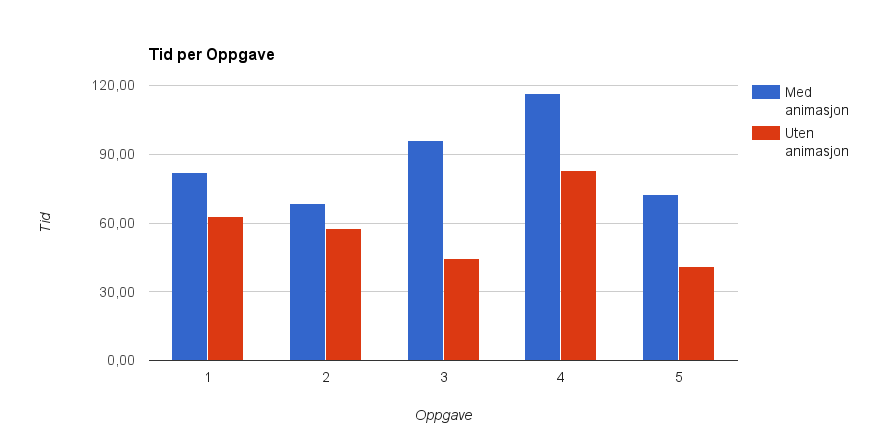
\includegraphics[width=100mm]{TidPerOppgave} 
\caption{Gjennomsnittlig tid per oppgave basert på om animasjoner var på eller ikke.} 
\label{fig:DiagramTidPerOppgave} 
\end{figure} 
 
 
I Diagrammet \ref{fig:DiagramTidPerOppgave} viser den blå søylen den gjennomsnittlige tiden det tok for deltakerne som hadde på animasjoner å gjennomføre oppgaven, mens den røde viser hvor lang tid det tok for de uten. Som man kan se utfra diagrammet, ser man at tendensen er at de som hadde på animasjoner brukte lengre tid en de uten. Dette kan tyde på at en bruker lengre tid ved å ha animasjonene slått på.  
 
 
 
\section{Tolkning av resultat} 
 

Det er viktig å poengtere at testen kun hadde 6 deltakere, noe som ikke gir grunnlag for konklusjon og dataene vil i beste fall kun gi indikasjoner.  Med testingen ønsket vi å undersøke hvorvidt målgruppen greide å utføre de mest nødvendige oppgavene i prototypen og hvilken påvirkning animasjoner og lyd hadde på barnet.  
 
Deltakerne hadde ingen erfaring med bruk av øyesporingsenheten eller lignende programvare. Allikevel tok det ikke lang tid før de tilpasset seg og trykket på de forskjellige symbolene. De hadde ingen spørsmål rundt hva som ble regnet som et klikk eller hva de ulike menyknappene betydde. Deltakerne greide også å gjennomføre alle oppgavene de ble tildelt. En liten tendens ble derimot oppdaget. Det var at alle deltakerne hadde problemer med timeren som viser hvor lenge det er igjen til en interaksjon blir regnet som et trykk. Hver gang denne dukket opp og nedtellingen startet, ble deltakeren stresset og flyttet blikket febrilsk rundt for å unngå feiltrykk. Dette var også en erfaring som ble gjort under testingen på medstudenter.  Det var derimot ikke nok til å hindre deltakerne i å operere programvaren og gjennomføre alle oppgavene.

Spørsmålet blir da hvorvidt man kan si om barn med funksjonsnedsettelse kunne utført de mest nødvendige operasjonene på prototypen. Selv om testeten hadde blitt utført på målgruppen hadde dette vært en usikkerhetsfaktor, ettersom det finnes flere funksjonshemninger og flere grader av dem. Det man kan si utfra testingen er at barn i 6 års alderen har ingen store problemer med å skrive og finne frem til de korrekte ordene. Vi kan derfor fastslå at et barn i målgruppen også vil hatt mulighet om ikke like lett kunne uttrykke seg selv gjennom prototypen. 
 
I tillegg vil testen også finne ut hvilken effekt animasjoner og lyd ville ha. For å finne ut dette ble data samlet inn mens deltakerne utførte 6 oppgaver som ble tildelt. Dataene er presentert i diagram og gir klare indikasjoner på at deltakerne som hadde animasjoner og lyd brukte lengre tid på oppgavene enn de uten. Dette er interessant, men det skal igjen nevnes at i tillegg til at det kun var 6 deltakere, var det også kun 6 oppgaver. Til tross for at de brukte lengre tid på å gjennomføre oppgavene, var det kun de 2 av 3 som hadde animasjoner på som kunne svare hva som skjedde ved å trykke på en kategori- og ordsymbol. Hvis dette skulle stemme, kan det tyde på at en bruker kanskje burde starte med å ha animasjoner på for etter en stund skru de av.  
 
Som en oppsummering kan en si at med såpass få testpersoner kan man ikke si noe sikkert, men vi kan konkludere med at prototypen fungerer og at et barn i seks år alderen enkelt greier å uttrykke seg via denne. I tillegg er det indikasjoner på at animasjoner gjør at en ny bruker av programvaren bruker lengre tid enn uten animasjoner. Det er også indikasjoner på animasjoner og lyd gir brukeren en bedre forståelse for hva de ulike typene symbol representerer.  
 

 

 
 
 
 
 
 
 
 
 
 
 
 

\chapter{Konklusjon}

\section{Konklusjon}

Oppgaven har bestått av to delmål. Det første var å utvikle en high-fidelity prototype. Det andre var å implementere ulike animasjoner og legge til lyder for å se hvilken innvirkning dette hadde på den tiltenkte målgruppen. Vi skulle også gjøre det mulig for en bruker å  tilpasse programmet ved øyesporing. 

1) Vi har utviklet en high-fidelity prototype som lar en bruker sette sammen enkle setninger. Den er kompatibel med en øyesporingsenhet som gjør at en bruker kan navigere ved å kun bruke øyene. En som tar i bruke denne interaksjonsformen har tilgang på alle de samme funksjonene som en datamus bruker. Når en bruker har skrevet en setning har mulighet for å presentere dette som lyd. Ettersom programmet er tiltenkt barn, er vært ord representert med et symbol. En utvikler kan enkelt bytte ut eller legge til nye ord og symboler ved å legge de inn i den medfølgende tekstfilen. Programmet er bygget på en moderne teknologi og har en kodekvalitet som gjør at den kan brukes i av andre i fremtidige prosjektet. Det er også mulighet for å videreutvikle prototypen til en ferdig programvare. 

2) I prototypen har vi lagt til flere animasjoner og lyder for å forbedre brukervennligheten. Vi har implementert ulike animasjoner og lagt til forskjellige lyder for differensiere mellom de ulike brikkene. Vi har også gjort det mulig for en bruker å tilpasse ulike aspekter i programmet etter egne ønsker. Dette er også mulig ved bruk av øyesporing. 

For å finne ut hvilken påvirkning dette hadde å brukerene ble det foretatt testing. Vi fikk ikke til å rekruttere folk som bruker Sono Flex eller lignende systemer til dagligdags. Dette gjorde at testen ble foretatt på barn i samme aldersgruppe på målgruppen. Testingen viste indikasjoner på at animasjoner og lyd gir brukeren en bedre forståelse av programvaren. Men får å kunne konkludere må det mer omfattende testing til.


\section{Videre arbeid}

\textbf{Omfattende testing}
I oppgaven har vi hatt vanskeligheter med å rekruttere testere. Først og fremst ble det ikke mulighet for å teste på målgruppen, altså barn i alderen 6 år som dagligdags bruker programvare til kommunikasjon. Og de deltakerne vi fikk, var ikke nok til å konkludere. Det vi derimot fikk, var vage indikasjoner. Så for å få bekrefte eller avkrefte disse, må det mer omfattende testing til. 


\textbf{Internasjonalisering}

\textbf{Legg til talespråk}
Foreløpig er naturlig tale kun tilgjengelig på engelsk. Det er enkelt å legge til flere språk i koden så lenge de er installert på maskinen. 

\textbf{Legg til flere innstillinger som  bruker kan endre}
Det er mulig for en bruker å tilpasse animasjonsfart, symbolstørrelse og temaer. Det burde derimot være mulighet for en bruker å endre mye mer ved kun øyestyring. Som for eksempel mulighet til å designe egne kategorier og flytte symboler. 

\textbf{Hva som skal til for videre bruk} 
Den viktigste funksjonaliteten er tilgjengelig i prototypen og den har blitt testet på barn og studenter. Men det er fortsatt mye som må gjøres for at den kan sies å være ferdig. Blant annet så har Sono Flex mye funksjonalitet som fortsatt ikke er implementert i prototypen. Den har blitt testet, men ikke på brukere som faktisk har behov for den. Så videre arbeid for å ferdigstille prototypen bør fokusere på implementasjon av manglende funksjonalitet og testing på målgruppen.

\textbf{Kategorisering og organisering}
En del av oppgaven var å se på optimal kategorisering og organisering. Dette har det desverre ikke blitt tid til, ettersom dette viste seg å være mer omfattende en først tiltenkt. Men for at et barn effektivt skal kunne bruke Sono Flex eller lignende programvare mer effektivt, bør dette feltet utforskes mer.


Mye av denne oppgaven er basert på videre arbeid, eller legge til rette for videre arbeid. Det kan sies at vi har laget en plattform for videre arbeid som både Tobii og fremtidige studenter kan forske på.


Prototypen inneholder funksjonalitet som gjør at den fungerer, den har blitt testet og både på barn og studentet, med og uten øyesporing. Allikevel vil det alltid dukke opp bugs og fail og v

Brukertilpasning er det mye som mangler

Lag tester til koden. 

Videre testing av de allerede implementere animasjonene

Hva skal til for at det er en ferdig programvare.
    - Legge til flere brikker, dette er enkelt.
    - Sono flex har mange flere funksjoner som ikke er tilgjengelig. Disse må implementeres. 
    - Mye mer testing.
    - 


Som en oppsummering så kan en si at med så lite testpersoner så kan man ikke si noe sikkert, men vi kan konkludere med at prototypen fungerer og at et barn i seks år alderen enkelt greier å uttrykke seg via denne. I tillegg er det indikasjoner på at animasjoner gjør at en ny bruker av programvaren bruker lengre tid enn uten animasjoner. Det er også indikasjoner på animasjoner og lyd gir brukeren en bedre forståelse for hva de ulike typene symbol representerer.  

For å utforske mulige løsninger som kan øke brukervennligheten til Sono Flex  vil en rekke funksjoner og design implementeres og testes. 

Hovedsakelig skal vi se på hvordan ulike elementer kan hjelpe en bruker i å finne ønsket symbol raskere. For eksempel hva vil gjøre at et barn enklere husker hvilken kategori han må trykke på for finne ønsket symbol. For å gjøre dette vil fokuset ligge på audiovisuelle hjelpemidler, men det vil også ses på hvordan en bør organisere de forskjellige ordene nedenfor. Listen nedenfor gir en  beskrivelse av det vi ønsker å utforske.



fungerer sammen med en øyesporingsenhet og mus, slik at en bruker kan velge alle funksjoner som er tilgjengelig for mus er også tilgjengelig ved åp kun bruke øyet.

Programmet er bygget på en moderne teknologi som gjør at den enkelt kan brukes i fremitdige prosjekter blant annet for masterstudenter eller for selskapet. Det er også mulighet for å ferdigstille den til et ferdig produkt.-



Vi har utviklet en prototype som lar barn sette sammen enkle setninger kun ved hjelp av øyene. Prototypen har kommet som et resultat av at den eksisterende løsningen, Sono Flex, er implementert i en teknologi ikke var kvalifisert for det vi ønsket å utforske i andre del. En stor del av oppgaven ble derfor å utvikle denne fra bunn av. Tobii så også muligheten til at dette kunne bli en plattform for fremtidige oppgaver og muligens starten på en ferdig programvare. 
























Den endelige koden er derfor av god kvalitet og det skal være mulig for andre utviklere å forstå og dermed videreutvikle. 


2) I prototypen har vi implementert de fleste komponentene som vi på forhånd ønsket å utforske. 


//Utviklet animasjoner og lyder


//Lar barn bruke øyesporing til å kommunisere, snakker med øyesporingsenheten.
//Koden har ved bruk av mønster, kodekonvesjoner og generelt betenksom rundt koding holdt en god kode.
//Tar i bruk de eksisterende symbolene.
//enkelt å legge til nye symboler.




Tobii Dynavox ønsket teste programvaren på en ny teknologi 

mulige forbedringer på en av deres programvarer. I dette tilfelle Sono Flex. Problemet var at den teknologien som denne er implementer i, holder på å bli utfaset. Derfor ble oppgaven todelt. Eller ret


Oppgaven gikk opprinnelig kun ut på å utforske mulige forbedringer vi kunne gjøre på den programvaren Sono Flex. 


Målet med denne oppgaven var todelt, først måtte vil utvikle en high-fidelity prototype med å


Målet med oppgaven har derfor blitt todelt. Det vil si at i tillegg til å bygge ut funksjoner og teste disse på den eksisterende programvaren, vil også programvaren som disse skal fungere på utvikles. Første delmål av oppgaven vil derfor være å utvikle programvaren. Andre delmål vil være å teste ulike design og funksjoner.


I oppgaven har vi gjort to ting, vi har laget en high-fidelity prototype 































I dette kapittelet vil vi først evaluere de to delmålene som er presentert i det første kapittelet. Her vil vi også komme med forslag til videre arbeid. Til slutt vil det være en konklusjon.

\section{Prototype}

Første del av oppgaven var å utvikle en high-fidelity prototype med fokus på hovedfunksjonaliteten til Sono Flex. Som vil si at den ligner svært mye et ferdig produkt med mye detaljer og funksjonalitet. Dette gjør at en kan foreta konklusjoner om oppførselen til det ferdige produktet. Grunnen til at det måtte utvikles en prototype istedenfor å videreutvikle på den eksisterende var:

- Teknologien som den eksisterende programvare Sono Flex er bygget på, er ikke tilrettelagt for animasjoner. Noe som var en viktig del av oppgaven.

- Den er også blitt satt i vedlikeholds modus av utvikleren Microsoft. Som vil si at feil og bugs vil bli rettet opp, men at det vil ikke komme nye funksjonalitet. Et tegn som kan tyde på at den fases ut.

Prototypen ble utviklet på WPF en teknologi som har eksistert lenge nok til at den er moden samtidig som den fortsatt blir utviklet av Microsoft. Teknologien ble valgt 







//Valget falt på WPF ligger tett opp til den eksisterende teknologien, men er bedre Støtte for hardware

//Kodekvalitet, fulgt kodestandarder, mønster som passer til teknologi. 


a prototype that is quite close to the final product, with lots of detail and functionality. From a user testing point of view, a high-fidelity prototype is close enough to a final product to be able to examine usability questions in detail and make strong conclusions about how behavior will relate to use of the final product.




\medskip

\bibliographystyle{chicago}%Used BibTeX style is unsrt
\bibliography{sample}

\end{document}
